\documentclass[paper=a4, fontsize=11pt]{scrartcl}

\usepackage{url}    
\usepackage[margin=1in]{geometry}
\setlength{\parskip}{0.5em}

% cref command
\usepackage[noabbrev,capitalise]{cleveref}

\usepackage[T1]{fontenc}
\usepackage{fourier}
\usepackage[english]{babel}
\usepackage{amsmath,amsfonts,amsthm}

\usepackage{sectsty} % Allows customizing section commands
\allsectionsfont{\centering \normalfont\scshape} % Make all sections centered, the default font and small caps

\usepackage{fancyhdr} % Custom headers and footers
\pagestyle{fancyplain} % Makes all pages in the document conform to the custom headers and footers
\fancyhead{} % No page header - if you want one, create it in the same way as the footers below
\fancyfoot[L]{} % Empty left footer
\fancyfoot[C]{} % Empty center footer
\fancyfoot[R]{\thepage} % Page numbering for right footer
\renewcommand{\headrulewidth}{0pt} % Remove header underlines
\renewcommand{\footrulewidth}{0pt} % Remove footer underlines
% \setlength{\headheight}{1pt} % Customize the height of the header

\numberwithin{equation}{section} % Number equations within sections (i.e. 1.1, 1.2, 2.1, 2.2 instead of 1, 2, 3, 4)
\numberwithin{figure}{section} % Number figures within sections (i.e. 1.1, 1.2, 2.1, 2.2 instead of 1, 2, 3, 4)
\numberwithin{table}{section} % Number tables within sections (i.e. 1.1, 1.2, 2.1, 2.2 instead of 1, 2, 3, 4)

\setlength\parindent{0pt} % Removes all indentation from paragraphs - comment this line for an assignment with lots of text


%----------------------------------------------------------------------------------------
%  TITLE
%----------------------------------------------------------------------------------------

\newcommand{\horrule}[1]{\rule{\linewidth}{#1}} % Create horizontal rule command with 1 argument of height

\title{	
    \normalfont
    \large \textsc{University of Groningen \\ Visual Analytics for Big Data} \\ [22pt]
    \horrule{0.5pt} \\[0.4cm]
    \huge Practical Assignment: \\ Visualizing Data with Tableau \\
    \horrule{0.5pt} \\[0.5cm]
}

\author{
    Davide Pedranz \\
    \small d.pedranz@student.rug.nl \\
    \small Student Number: S3543757    
}

\date{\vspace{0.5cm} \normalsize\today}

%----------------------------------------------------------------------------------------
%  DOCUMENT
%----------------------------------------------------------------------------------------

\begin{document}
\maketitle

\tableofcontents

\section*{Tableau Visualization}
TODO: put link here

\clearpage

\section{Exploring the incidents' geographical distribution}
\label{sec:question1}

\subsection*{Question 1.1}
\textit{Are there high variations of incidents densities over Seattle? Which are the low-density zones? Which are the high density zones?}

The visualization uses a map of the city of Seattle (a scatter plot that uses the maps from OpenStreetMap for the background):
each point in the dataset is visualized as a circle on the map.
Columns and rows are used to encode respectively longitude and latitude.
The size of the circles is set to the minimum, the opacity to the value $8\%$.
Size and opacity do not encode any particular information.
However, the combination of small size, opacity and zoom level allows to visualize an approximation of the density of incidents.
The zoom level is small in order to get an overview of the entire city that fits the screen.
Size and opacity are adjusted accordingly.

\begin{figure}[h]
	\centering
	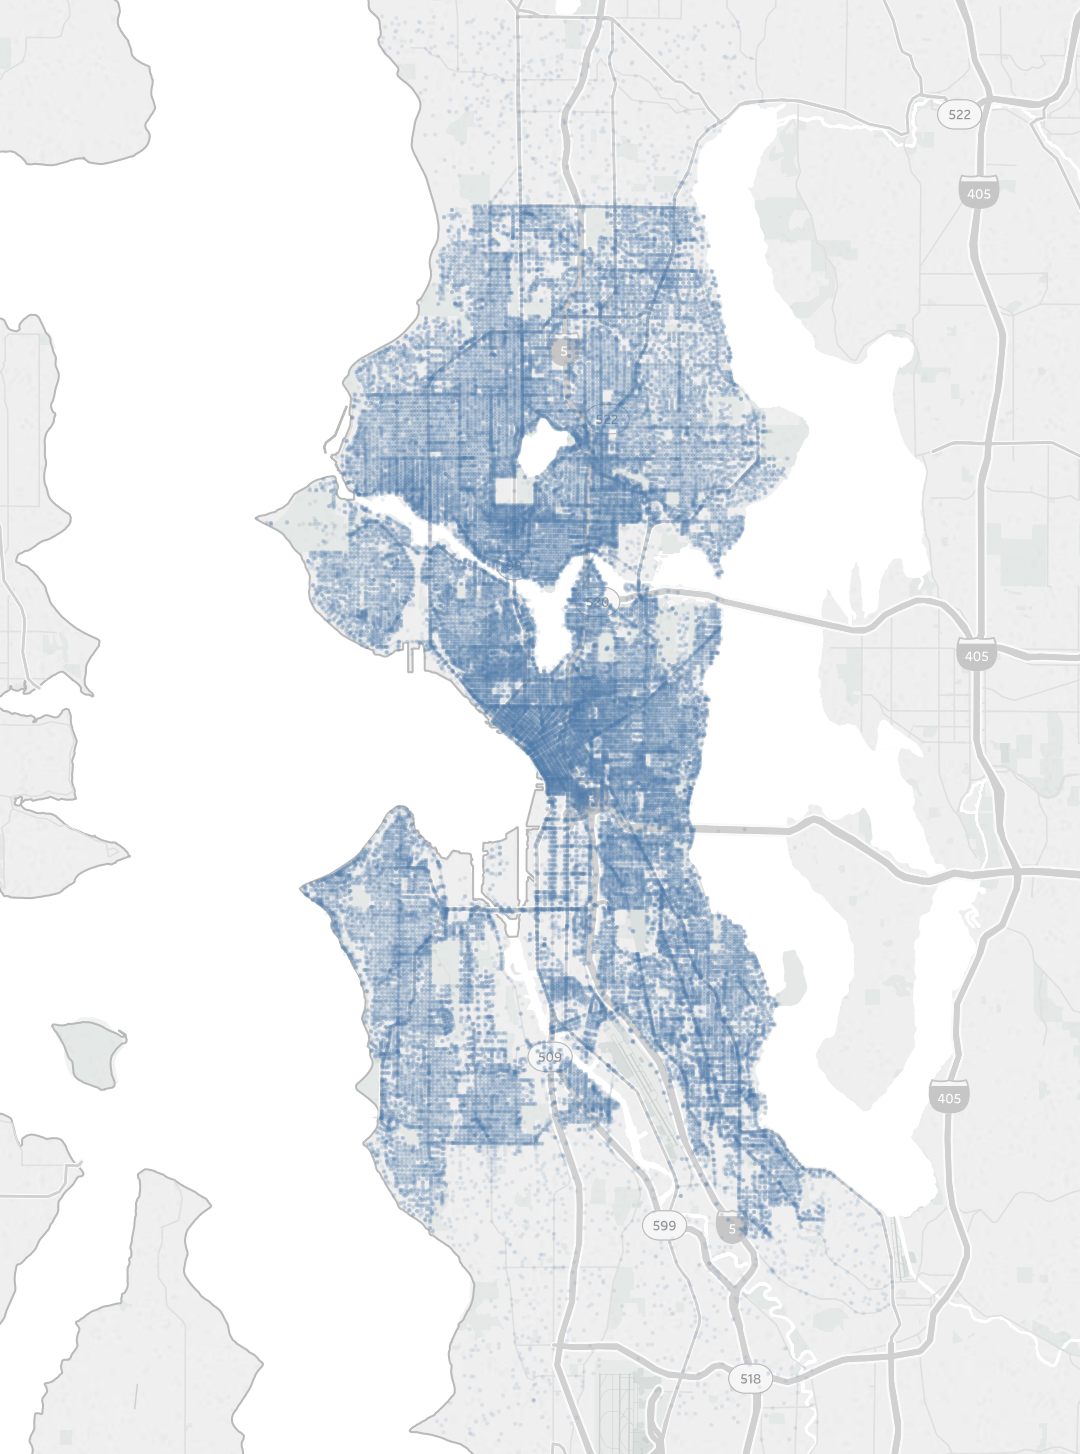
\includegraphics[width=.75\columnwidth]{figures/1_1_geographical_distribution_incidents}
	\caption{Geographical distribution of the incidents in Seattle. The screenshot is taken from the sheet called \textit{Geographical Distribution of Incidents in Seattle} in Tableau.}
	\label{fig:1_1_geographical_distribution_incidents}
\end{figure}

\cref{fig:1_1_geographical_distribution_incidents} shows that there are indeed variations in the density of incidents in Seattle:
\begin{itemize}
    \item The regions in the very north and south of the city have a very small number of incidents. These areas are already outside the borders of Seattle. We suspect they are not usually covered by the police of Seattle, so the dataset may not contain all the incidents that occurred in the those areas.
    \item Incidents seem to be more concentrated in the central area of the city, around the Elliott Bay, and immediately to its north.
    \item Outside the city center, the main roads have a higher number of incidents than the surrounding areas (in particular in the south part of the city).
    \item The density of incidents in the rest of the city is lower and seems to be approximately uniform.
\end{itemize}

The visualization answers the question, but it is not optimal.
A better solution would be to use a density plot which is able to visualize better the differences of incidents' densities in the city.
Unfortunately, Tableau does implement density plots: the proposed solution tries to approximate a density plot by finding the right level of opacity, size and zoom using Tableau.

\subsection*{Question 1.2}
\textit{Are there high variations of incidents densities over Seattle for specific types of incidents? Which are these types and which are the variations you found?}

\begin{figure}[h!] 
    \begin{subfigure}{0.5\textwidth}
        \centering
        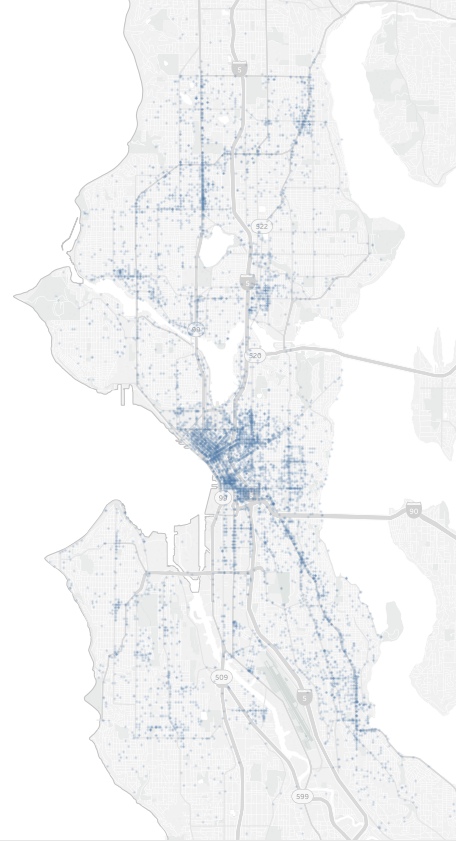
\includegraphics[width=0.8\linewidth]{figures/1_2_geographical_distribution_arrests} 
        \caption{Arrests}
        \label{fig:1_2_arrests}
    \end{subfigure}
    \begin{subfigure}{0.5\textwidth}
        \centering
        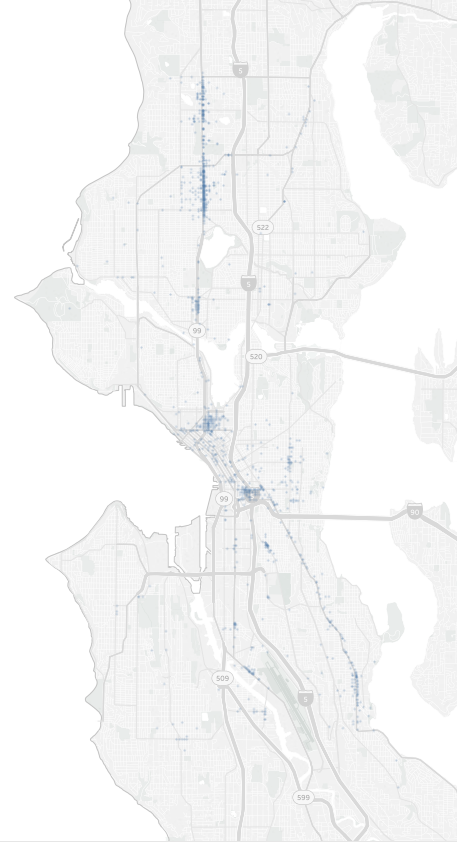
\includegraphics[width=0.8\linewidth]{figures/1_2_geographical_distribution_prostitution}
        \caption{Prostitution}
        \label{fig:1_2_prostitution}
    \end{subfigure}
    \caption{Geographical distribution of the incidents of type \textit{arrest} (on the left) and \textit{prostitution} (on the right) in Seattle. The screenshots are taken from the sheet called \textit{Sheet 22} in Tableau.}
    \label{fig:1_2_geographical_distribution_by_type}
\end{figure}

The visualization uses an approach similar to the previous section, but exploits pagination to display the different types of incidents individually.
This is done by using the ``Pages'' option in Tableau:
it is possible to interactively change the type visualized by using the dedicated menu.
The visualization uses a filter to exclude the observations without a type.
Since there are less observations in each page, the opacity value is set to a higher value ($30\%$).

\cref{fig:1_2_geographical_distribution_by_type} shows $2$ snapshots for the types \textit{arrest} and \textit{prostitution}.
From the figure it is already possible to notice that different types of incidents have different distributions in the city.
\cref{tab:distribution_by_type} contains the observations for every type of incident.

\renewcommand{\arraystretch}{1.5}
\begin{longtable}{ | >{\arraybackslash} m{5cm} | >{\arraybackslash} m{10cm} | }
    \hline
    \textbf{Incident Type} & \textbf{Description} \\
    \hline
    Accident Investigation  &   Higher concentration in the city center. Outside the city center, main roads have a higher concentration than the surrounding areas. \\
    \hline        
    Animal Complaints       &   Slightly higher concentration in the city center. \\
    \hline
    Arrest                  &   Higher concentration in the city center and along main roads in the north and south of the city. \\
    \hline
    Assaults                &   Like \textit{Arrest}. \\
    \hline
    Auto Thefts             &   No significant variations. \\
    \hline
    Behavioral Health       &   Higher concentration in the city center. \\
    \hline
    Bike                    &   Higher concentration in the city center. The north has a higher concentration thant the south. \\
    \hline
    Burglary                &   No significant variations. \\
    \hline
    Car Prowl               &   Slightly more concentrated in the city center. \\
    \hline
    Disturbances            &   Like \textit{Car Prowl}. \\
    \hline
    Drive By (No Injury)    &   Higher concentration in south east, almost absent in the other sectors. \\
    \hline
    Failure to Register (Sex Offender) &   Slightly more concentrated in the city center and south east. \\
    \hline
    False Alacad            &   No significant variations. \\
    \hline
    False Alarms            &   No significant variations. \\
    \hline
    Fraud Calls             &   Like \textit{Car Prowl}. \\
    \hline
    Harbor Calls            &   Concentrated along the coast. \\
    \hline
    Hazards                 &   Like \textit{Arrest}. \\
    \hline
    Homicide                &   Slightly more concentrated in the city center. \\
    \hline
    Lewd Conduct            &   Higher concentration in the city center. \\
    \hline
    Liquor Violations       &   Like \textit{Arrest}. \\
    \hline
    Miscellaneous Misdemeanors &   Like \textit{Arrest}. \\
    \hline
    Motor Vehicle Collision Investigation &   More concentrated in the center and along the streets. \\
    \hline
    Narcotics Complaints    &   Like \textit{Arrest}. \\
    \hline
    Nuisance, Mischief      &   Like \textit{Arrest}. \\
    \hline
    Other Property          &   Like \textit{Arrest}. \\
    \hline
    Person Down / Injury    &   Higher concentration in the city center. \\
    \hline
    Persons - Lost, Found, Missing &   Slightly more concentrated in the city center. \\
    \hline
    Property - Missing, Found    &   Slightly more concentrated in the city center. \\
    \hline
    Property Damage         &   Like \textit{Arrest}. \\
    \hline
    Prostitution            &   Concentrated along the main streets in the north and in the south. Present also in the city center. \\
    \hline
    Prowler                 &   No significant variations. \\
    \hline
    Public Gatherings       &   Higher concentration in the city center. \\
    \hline
    Reckless Burning        &   No significant variations. \\
    \hline
    Robbery                 &   Like \textit{Arrest}. \\
    \hline
    Shoplifting             &   Like \textit{Arrest}. \\
    \hline
    Suspicious Circumstances &   No significant variations. \\
    \hline
    Threats, Harassment     &   Like \textit{Arrest}. \\
    \hline
    Traffic Related Calls   &   No significant variations. \\
    \hline
    Trespass                &   Like \textit{Arrest}. \\
    \hline
    Vice Calls              &   No significant variations. \\
    \hline
    Weapon Calls            &   Like \textit{Arrest}. \\
    \hline

    \caption{Distribution of incidents in Seattle by type.}
    \label{tab:distribution_by_type}
\end{longtable}

The proposed visualization allows to analyze the distribution of incidents' types one by one.
However, it makes really difficult to compare different types, since the user needs to change page each time.

To overcome this limitation, we have to display different types together.
The first solution is to visualize all incidents together on the same map and use a categorical color map to distinguish them (see sheet \textit{Incidents Distribution (all types together)} in Tableau).
The user can interactively select subsets of types to display and filter out the others.
This solution presents $2$ main problems:
\begin{itemize}
    \item A categorical color map should use color which appear very different for each other to be useful, in the ideal case a set of color for which each pair has the same distance in RGB from each other. Unfortunately, it is impossible to find such a set for more than $4$ colors. We have about $40$ different types, so such an encoding is not effective.
    \item There are too many points, so even if we could find a good set of colors for the encoding, the point would overlap with each other. We can not use transparency to visualize also the underlying points since, since colors would mix together and create new ones.
\end{itemize}

One could use the following approaches to solve the problem:
\begin{itemize}
    \item Select a subset of types to show. Unfortunately, there is not an easy choice. Types with a higher number of incidents do not in general have an interesting distribution (i.e. their geographical distribution is similar to the one for all incidents). On the other hand, less frequent types have often a very interesting behaviour (see \textit{Prostitution}).
    \item Cluster similar types together. Unfortunately, it is not easy to build a types' hierarchy.
\end{itemize}

An alternative solution is to apply the small multiple design idea, i.e. create a visualization for a single type and replicate it multiple times.
This idea is implemented in sheet \textit{Incidents Distribution (small multiple design)} in Tableau:
each type is displayed on its own map, and maps for different types are shown in columns adjacent to each other (we use columns because the shape of the city on the chart is stretched out along the y-axis).
The type of incident in encoded both in space (different charts) and in color:
this overloading makes easier to distinguish different types.
Types are sorted in alphabetical order by default, but the user can interactively re-order them in order to compare $2$ or $3$ types at a time.
\cref{fig:1_2_geographical_distribution_comparison} shows an example of such a comparison:
types \textit{Prostitution}, \textit{Drive by} and \textit{Failure to register (self offender)} seem to be somehow correlated in the south-east part of the city but not in the north.
The size of each point is chosen to be small, but the opacity is set larger than for Question 1.1 since there are fewer point in each map.

\begin{figure}[h]
	\centering
	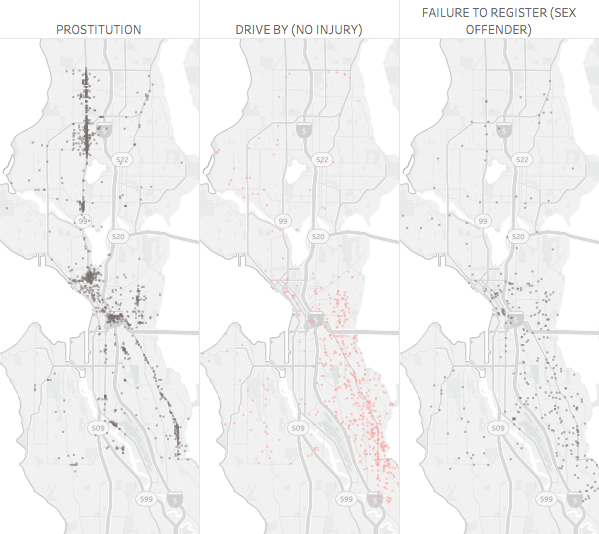
\includegraphics[width=.75\columnwidth]{figures/1_2_geographical_distribution_comparison}
	\caption{Geographical distribution of incidents of types \textit{Prostitution}, \textit{Drive by} and \textit{Failure to register (sex offender)} in Seattle. The screenshot is taken from sheet \textit{Incidents Distribution (small multiple design)} in Tableau.}
	\label{fig:1_2_geographical_distribution_comparison}
\end{figure}

\section{Exploring the incidents' geographical and temporal distribution}
\label{sec:question2}

\subsection*{Question 2.1}
\textit{Do you see a different spatial distribution of incidents over the different years? If so, which are the differences you found?}

Before trying to answer this question, it is interesting to take a closer look to the data.
The data span a temporal period of $9$ years, from $2009$ to $2017$.
The dataset contains $1.441.208$ records, of which $1.027.546$ (about $70\%$) have no information about the time of the incident.
Also, there are only $7$ incidents for year $2009$ and $84$ for year $2010$ (we suspect that many incidents without the time information have happened in these years, but we have no evidence of that).
Our analysis concentrate thus on years $2011$ to $2017$.

Similar to Question 1.2, we use the small multiple design technique.
The visualization is composed of multiple maps: each map shows the incidents in Seattle for a single year.
The maps are sorted in chronological order, i.e. $2011$ is the first on the left, $2017$ the last on the right.
The user is free to change the order to make accurate comparison between pairs of years, if needed.
Since the visualization only shows data for $7$ years, it fits in a single screen.

We use a small size for each point on the map and a medium level of transparency to be able to distinguish areas with different densities.
We use color to overload the encoding of the year:
this allows to combine the visualization with the histogram of incidents' frequency by year, as shown in \cref{fig:2_1_geographical_temporal_distribution}.

\begin{figure}[H]
	\centering
	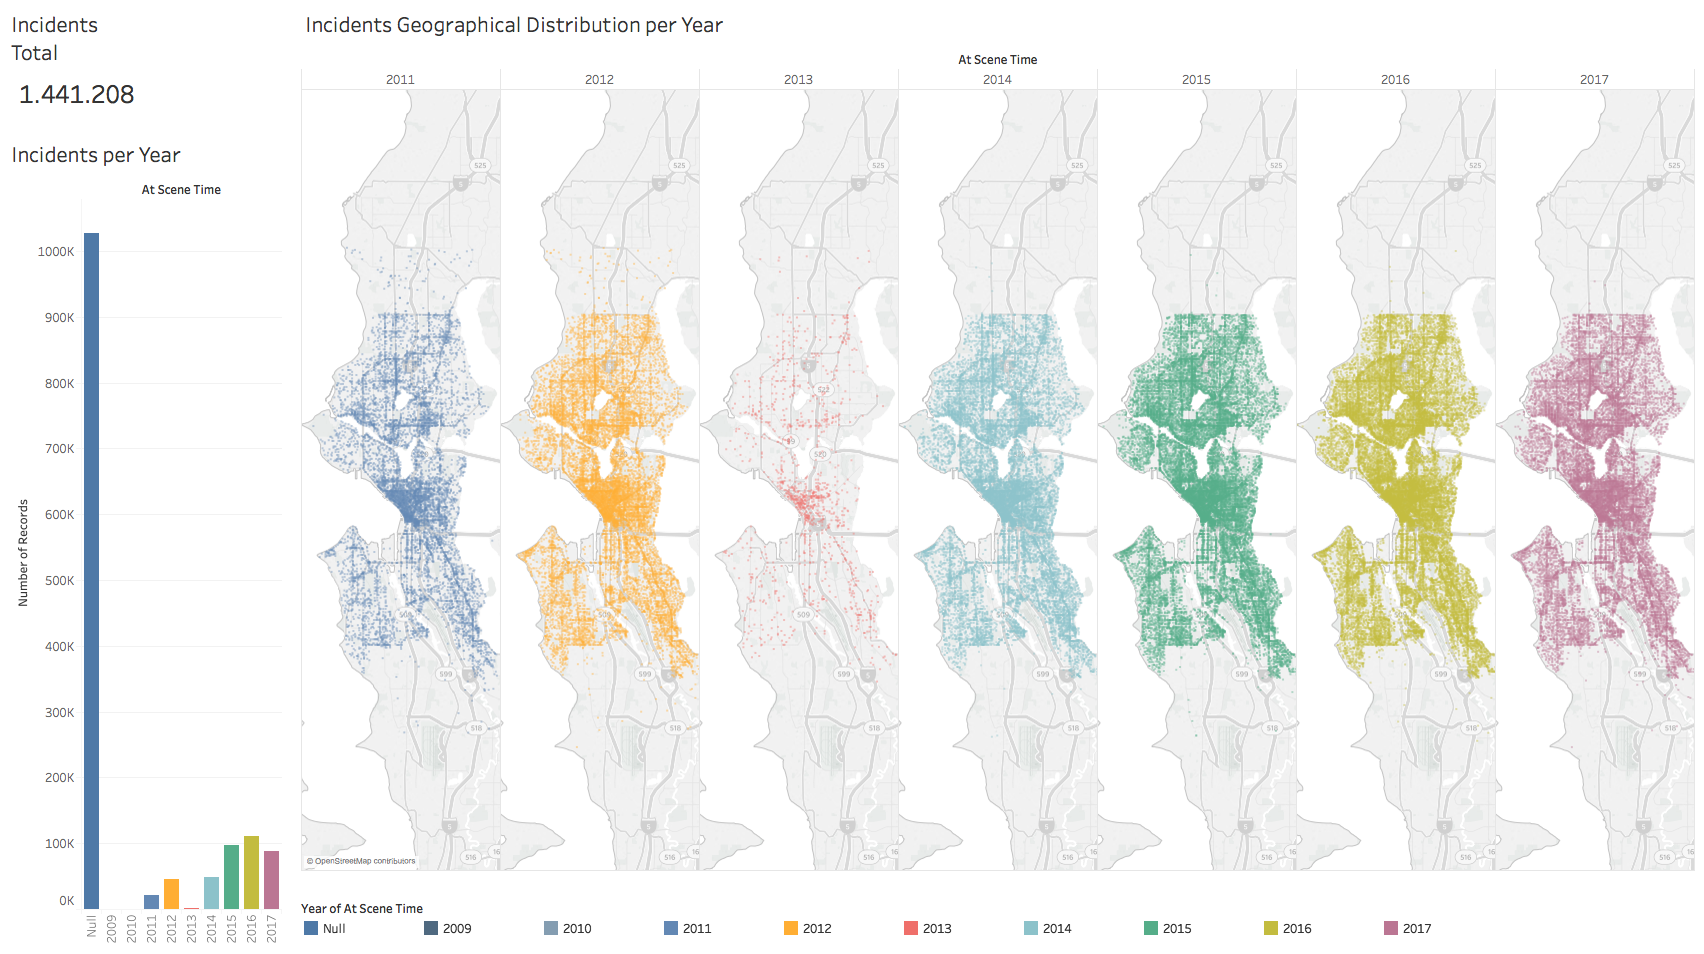
\includegraphics[width=\columnwidth]{figures/2_1_geographical_temporal_distribution}
	\caption{Incidents spatial distribution over different years in Seattle. The dashboard is called \textit{Incidents geographical and temporal distribution} in Tableau.}
	\label{fig:2_1_geographical_temporal_distribution}
\end{figure}

From the visualization, we can not notice any significant difference in the spatial distribution of incidents over the last $5$ years.
Year $2013$ has significantly less incidents, but this is probably due to the missing temporal information on $70\%$ of the entries.
Anyway, their distribution is similar to the general one: incidents are more concentrated in the city center (see Question 1.1).


\subsection*{Question 2.2}
\textit{Are there zones with a consistent low incidents density over all years? Are there zones with a consistent high density over all years?}

We can use the visualization built for the previous question to answer.
Over all years, the city center has a higher concentration of incidents.
Outside the city center, incidents seems to be slightly more concentrated along the main streets.
The distribution in each year is similar to the distribution over all years and is described in greater details in \cref{sec:question1}.

\section{Exploring the resolution speed}
\label{sec:question3}

\subsection*{Question 3.1}
\textit{What is the average resolution speed to an incident? Resolution speed is defined as the difference between the Event Clearance Date value (moment when the police closed the file of an incident) and the At Scene Time value (moment when the police arrived at the scene of the incident).}

The dataset does not define the average resolution time explicitly.
Thus, we need to add a new columns to the dataset with this information.
Tableau is able to compute new dimensions using the existing ones.
Since we compute a difference between $2$ timestamp, we use the function \texttt{datediff} to get a proper result.

The average resolution time of the entire dataset is about $2$ hours.

\begin{figure}[h]
	\centering
	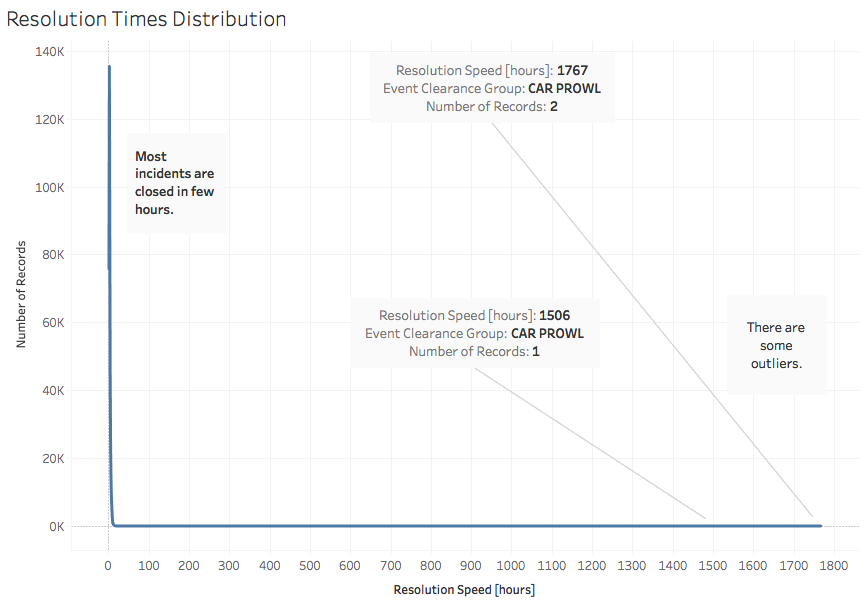
\includegraphics[width=0.9\columnwidth]{figures/3_1_resolution_speed_outliers}
	\caption{Distribution of the resolution times. The annotations on the plot show some outliers with very high resolution times. Most of the incidents are closed in few hours. This is a screenshot of sheet \textit{Resolution Times Distribution} in Tableau.}
	\label{fig:3_1_resolution_speed_outliers}
\end{figure}

\cref{fig:3_1_resolution_speed_outliers} shows the distribution of resolution times.
We can notice that:
\begin{itemize}
    \item Most incidents are closed in few hours.
    \item There are few outliers that have a resolution time of over $1500$ hours (approximately 2 months). All outliers share the same type: \textit{Car Prowl}.
\end{itemize}

The line chart gives already some interesting insides about incidents resolution times.
Due to the described outliers, it is difficult to read the left part of the chart, where most of the distribution mass is.

To solve the problem, we add an histogram of the resolution times.
Resolution time is a continuos measure, but we are not interested in the precise value for each incident, rather in the overall distribution.
To visualize the distribution, we discretize the resolution time in buckets of $1$ hour.
Since most of the density mass in the first $15$ buckets, we cut the histogram after the first $20$ ones.
Since we are loosing the outliers, we add a table that contains such information.

\cref{fig:3_1_resolution_speed} shows the final dashboard.
We can notice that:
\begin{itemize}
    \item The average resolution time is about $2$ hours.
    \item There are some outliers, but their number is really low in comparison to the amount of entries.
    \item Most incidents are closed in less than $10$ hours.
\end{itemize}

\begin{figure}[h]
	\centering
	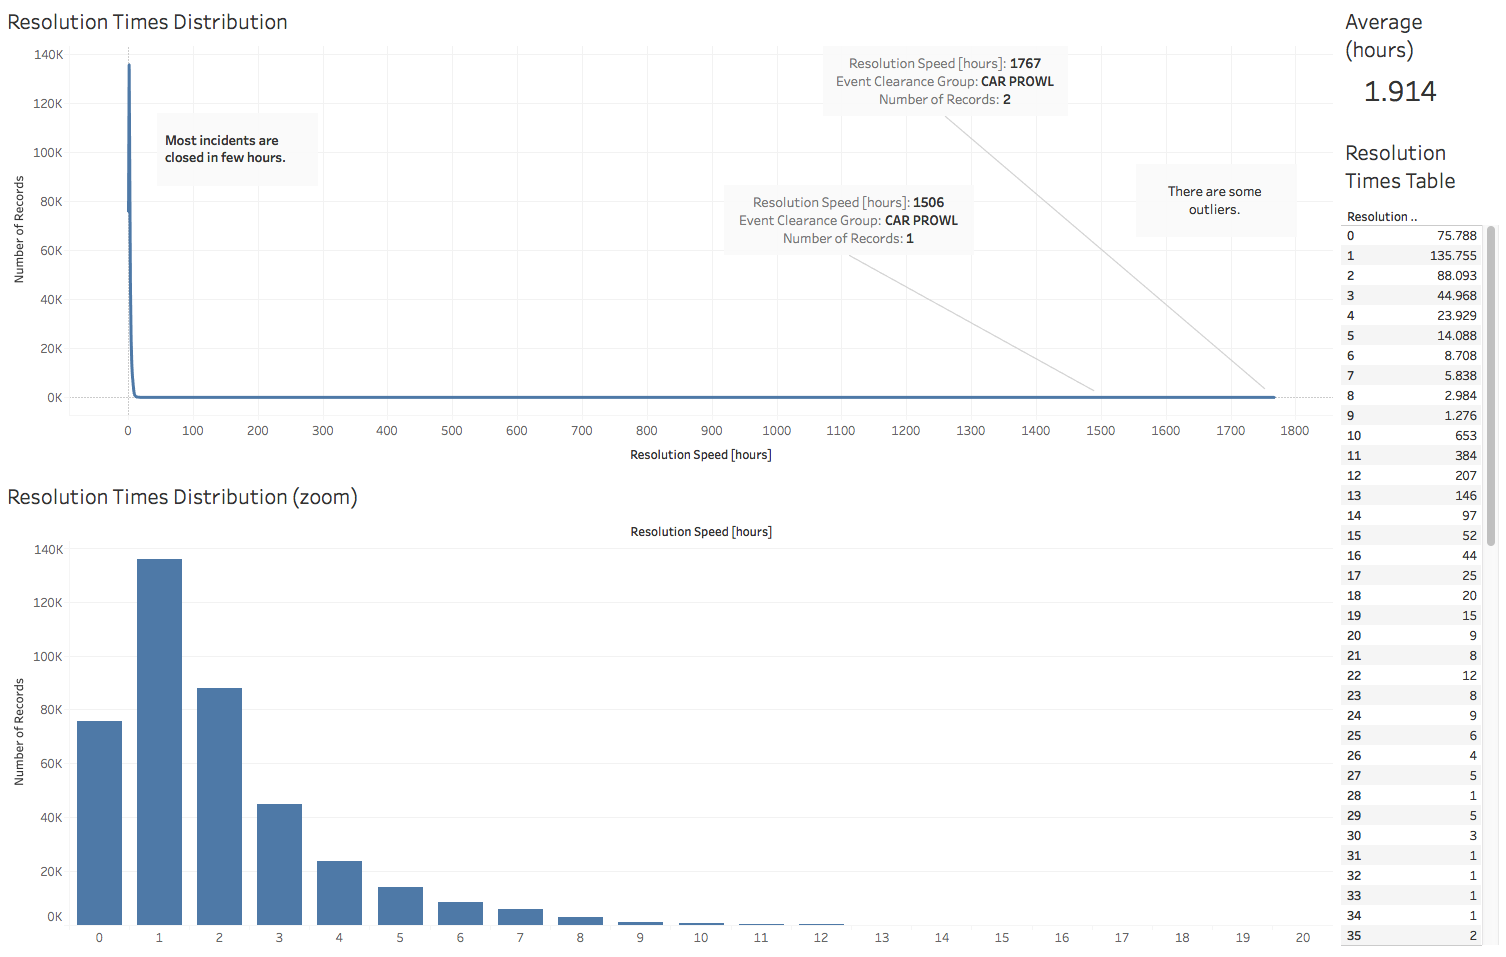
\includegraphics[width=\columnwidth]{figures/3_1_resolution_speed}
	\caption{Distribution of the resolution times. The dashboard is called \textit{Resolution Times} in Tableau.}
	\label{fig:3_1_resolution_speed}
\end{figure}


\subsection*{Question 3.2}
\textit{Are there certain types of incidents having a much lower resolution speed than others? If so, which are these?}

The visualization uses a bar chart.
Each type of is encoded in one bar and the height of the bar corresponds to the average resolution time for that type.
The types are ordered by average resolution time decreasing, so it is easy to spot the outliers.
Color is used to overload the encoding of the incident type.
The bar chart show the average line to make comparison and reasoning easier.
We prefer to use the x-axis for the type and the y-axis for the average resolution time since the visualization with swapped axises does not fit a single screen.

\cref{fig:3_2_resolution_speed_by_type} shows the visualization.
We can notice that:
\begin{itemize}
    \item \textit{Homicide} is the type with the highest average resolution time. This is not a surprise, since such an incident requires very accurate investigations.
    \item \textit{Public Gatherings} have the seconds highest average resolution time. This is probably due to the high number of people involved in the incident.
    \item \textit{Vice Calls} have the fastest resolution time, on average only about $30$ minutes.
    \item \textit{False Alarms} are also resolved quite fast, less than $1$ hour on average.
    \item All other types have resolution times between $1$ and $3$ hours on average.
    \item The distribution is skewed to towards types with higher resolution times.
\end{itemize}

\begin{figure}[h]
	\centering
	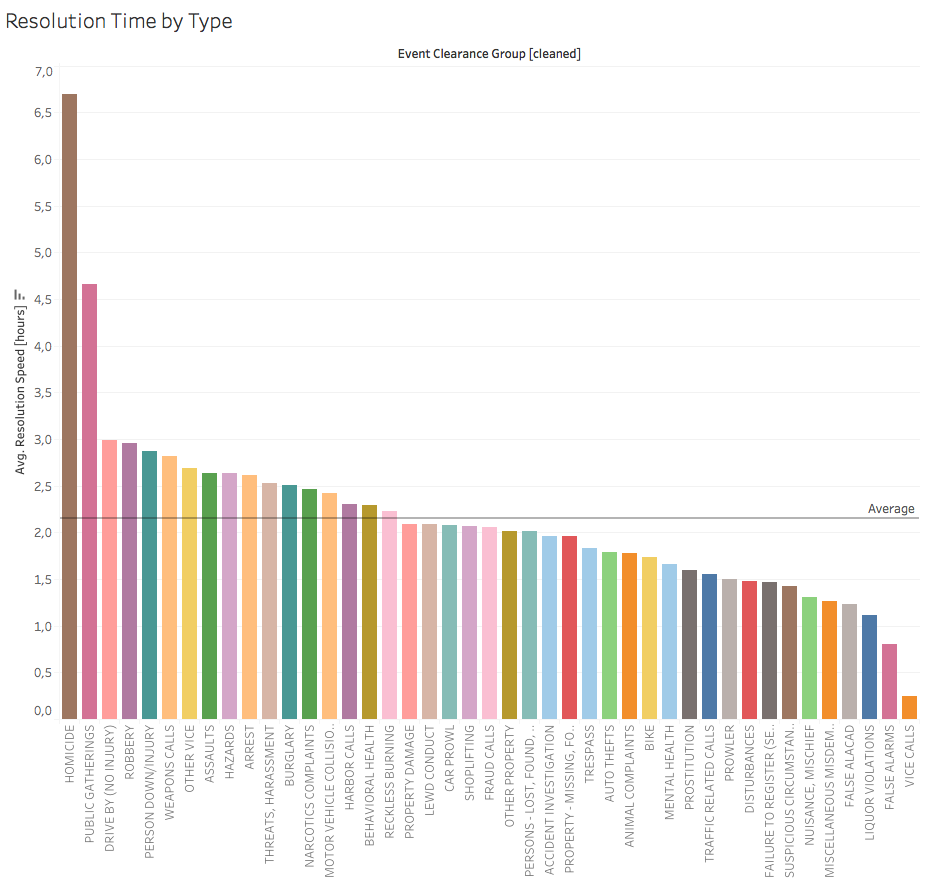
\includegraphics[width=\columnwidth]{figures/3_2_resolution_speed_by_type}
	\caption{Incidents' resolution time by type. The sheet is called \textit{Resolution Time by Type} in Tableau.}
	\label{fig:3_2_resolution_speed_by_type}
\end{figure}


\subsection*{Question 3.3}
\textit{Does the resolution speed depend on the time period (e.g., year, season of the year)?}

The visualization uses a Gantt chart to visualize the resolution speed of incidents over time.
The x-axis encode the time at scene, the y-axis the resolution speed in hours.
We use color to overload the encoding of the resolution speed.
In particular, we use a continuos heat colormap.
We show the average line in order to be able to compare time ranges with the average behaviour.

\begin{figure}[h]
	\centering
	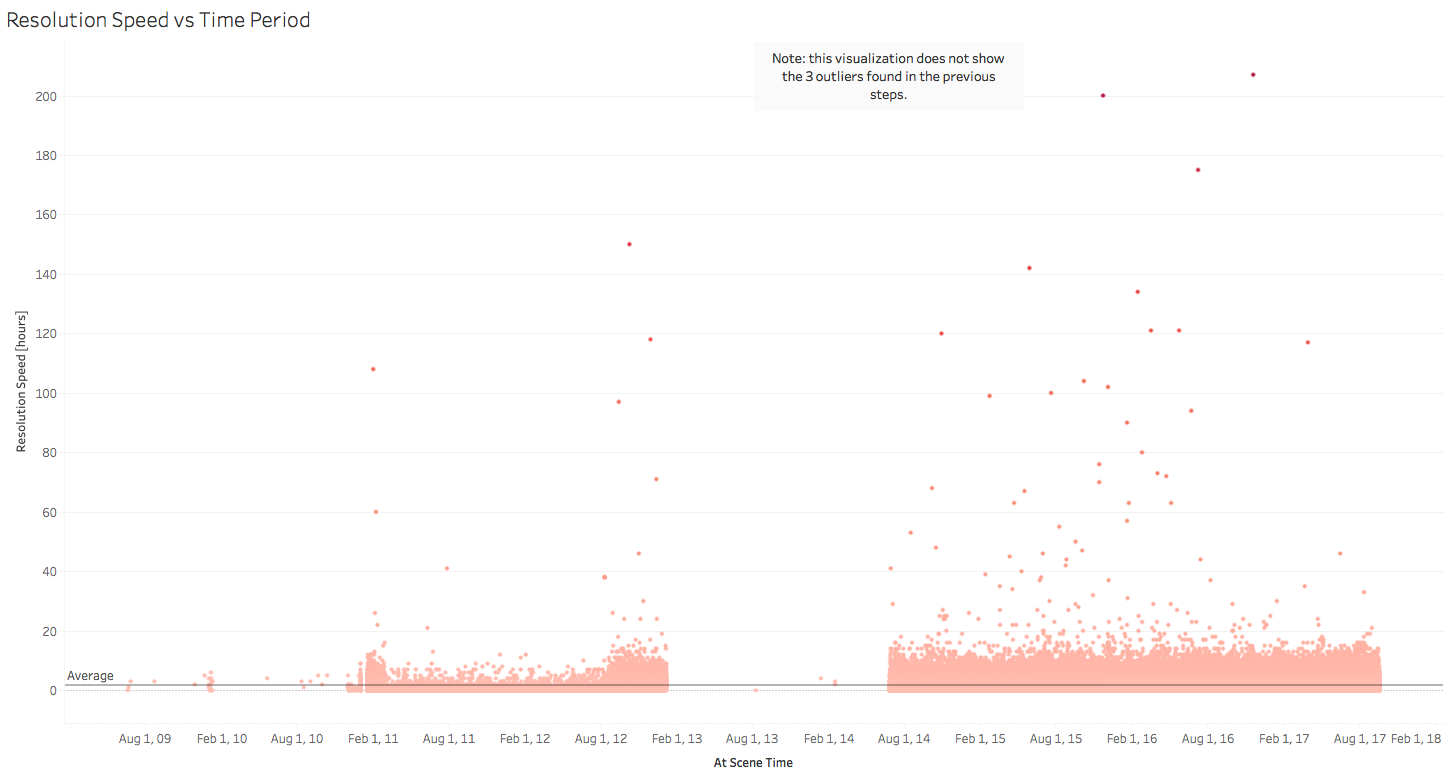
\includegraphics[width=\columnwidth]{figures/3_3_resolution_speed_vs_time}
	\caption{Incidents' resolution speed over time. Please note that the $3$ outliers cited in the text are excluded from this visualization. The sheet is called \textit{Resolution Speed vs Time} in Tableau.}
	\label{fig:3_3_resolution_speed_vs_time}
\end{figure}

The visualization is difficult to read due to the presence of the $3$ outliers described in Question 3.1.
Since we have discussed them already, we remove them from this visualization.
The result is shown is \cref{fig:3_3_resolution_speed_vs_time}:
\begin{itemize}
    \item There are $4$ slots of times that appears differently. The $1^{st}$ (02/2009 - 01/2010) and $3^{rd}$ (02/2013 - 07/2014) slots have almost no data. There is not much we can say about those periods.
    \item The $2^{nd}$ slot (02/2011 - 01/2013) has a period where incidents are resolved faster, in particular from 03/2011 to 08/2012; in this period most incidents are closed in less than $2$ hours.
    \item The $4^{th}$ slot (08/2014 - 09/2017) seems to have a uniform distribution for the resolution speeds, with an average higher than the $2^{nd}$ slot.
\end{itemize}

From \cref{fig:3_3_resolution_speed_vs_time} the resolution speed seems to be not correlated to the particular period of the year (i.e. month or season).
To confirm this hypothesis, we create $2$ new bar charts that show respectively the average resolution speed by season and by month (see \cref{fig:3_3_resolution_speed_by_season_and_month}):
there is no significant correlation between the period of the year and the incidents' resolution speed.
The Gantt chart and the $2$ bar charts are grouped in the \textit{Resolution Speed} dashboard.

\begin{figure}[h!]
    \begin{subfigure}{0.45\textwidth}
        \centering
        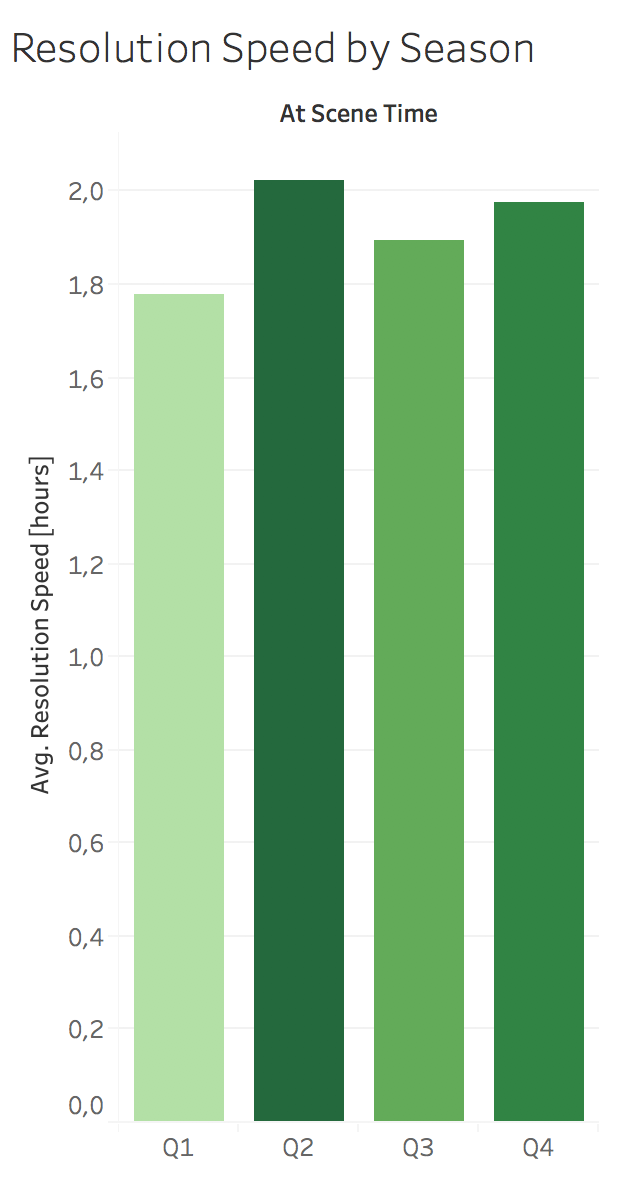
\includegraphics[width=0.342\linewidth]{figures/3_3_resolution_speed_by_season} 
        \caption{Resolution speed by season.}
        \label{fig:3_3_resolution_speed_by_season}
    \end{subfigure}
    \begin{subfigure}{0.55\textwidth}
        \centering
        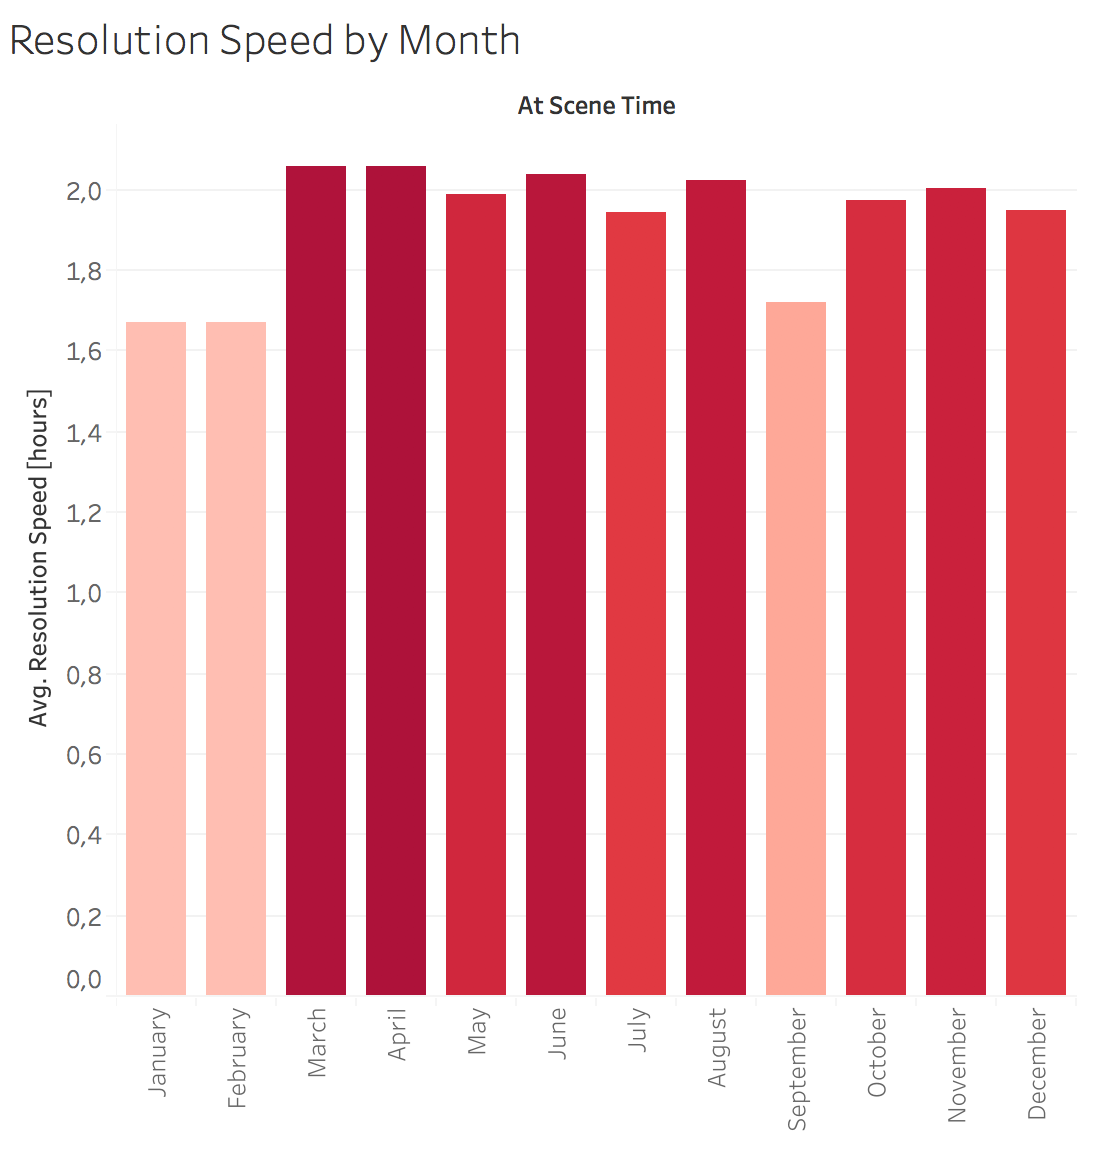
\includegraphics[width=0.7\linewidth]{figures/3_3_resolution_speed_by_month}
        \caption{Resolution speed by month.}
        \label{fig:3_3_resolution_speed_by_month}
    \end{subfigure}
    \caption{Resolution speed by season and month. The bar chart are grouped in the \textit{Resolution Speed} dashboard in Tableau.}
    \label{fig:3_3_resolution_speed_by_season_and_month}
\end{figure}

\section{Exploring the incidents' classification}

\subsection*{Question 4.1}
\textit{Incidents have two types: the type of the incident at the moment it was reported (Initial Type Group) and the type of the incident after it has been studied and classified (Event Clearance Group). Obviously, there should be some kind of correlation of the latter with the former (for instance, incidents reported as robberies are very likely to be also classified finally as robberies). How strong is this correlation?}

The visualization uses a heatmap to show this correlation.
The rows report the incident types at the moment it was reported, while the columns the type it was classified as (we will refer to it as the ``final'' type).
Each cell in the map contains a square, whose area and color are proportional to the number of record for the particular row and column.
Color uses a continuos heat colormap.

The order of rows and columns is initially alphabetical.
However, since there is no $1$-to-$1$ mapping between the categorical values of ``Initial Type Group'' and ``Event Clearance Group'', this order does not have any particular meaning.
Starting from such an order, we have moved some rows and columns to types which seems to be possibly correlated.
For example, ``Initial Type Group'' has the value \textit{Parking Violation}, but ``Event Clearance Group'' does not have it:
we have it closed to \textit{Traffic Related Calls}.

\cref{fig:4_1_initial_vs_final_group_heatmap} shows the visualization.
We can see that:
\begin{itemize}
    \item After some reordering of columns, most of the big squares are along the main diagonal. This means there is a very high correlation between the initial and final types of incidents.
    \item In many cases there is a $1$-to-$1$ match between the initial and final type (e.g. \textit{Disturbances}). In some cases a single initial type matches multiple more specific final types (e.g. \textit{Theft} matches with \textit{Car prowl}, \textit{Other property} and \textit{Shoplifting}).
    \item The first row of the table has a different behaviour. This row represent items without an initial type. They matches different final types, mostly \textit{Disturbances}, \textit{Suspicious circumstances} and \textit{Traffic related calls}.
\end{itemize}

\begin{figure}[h]
	\centering
	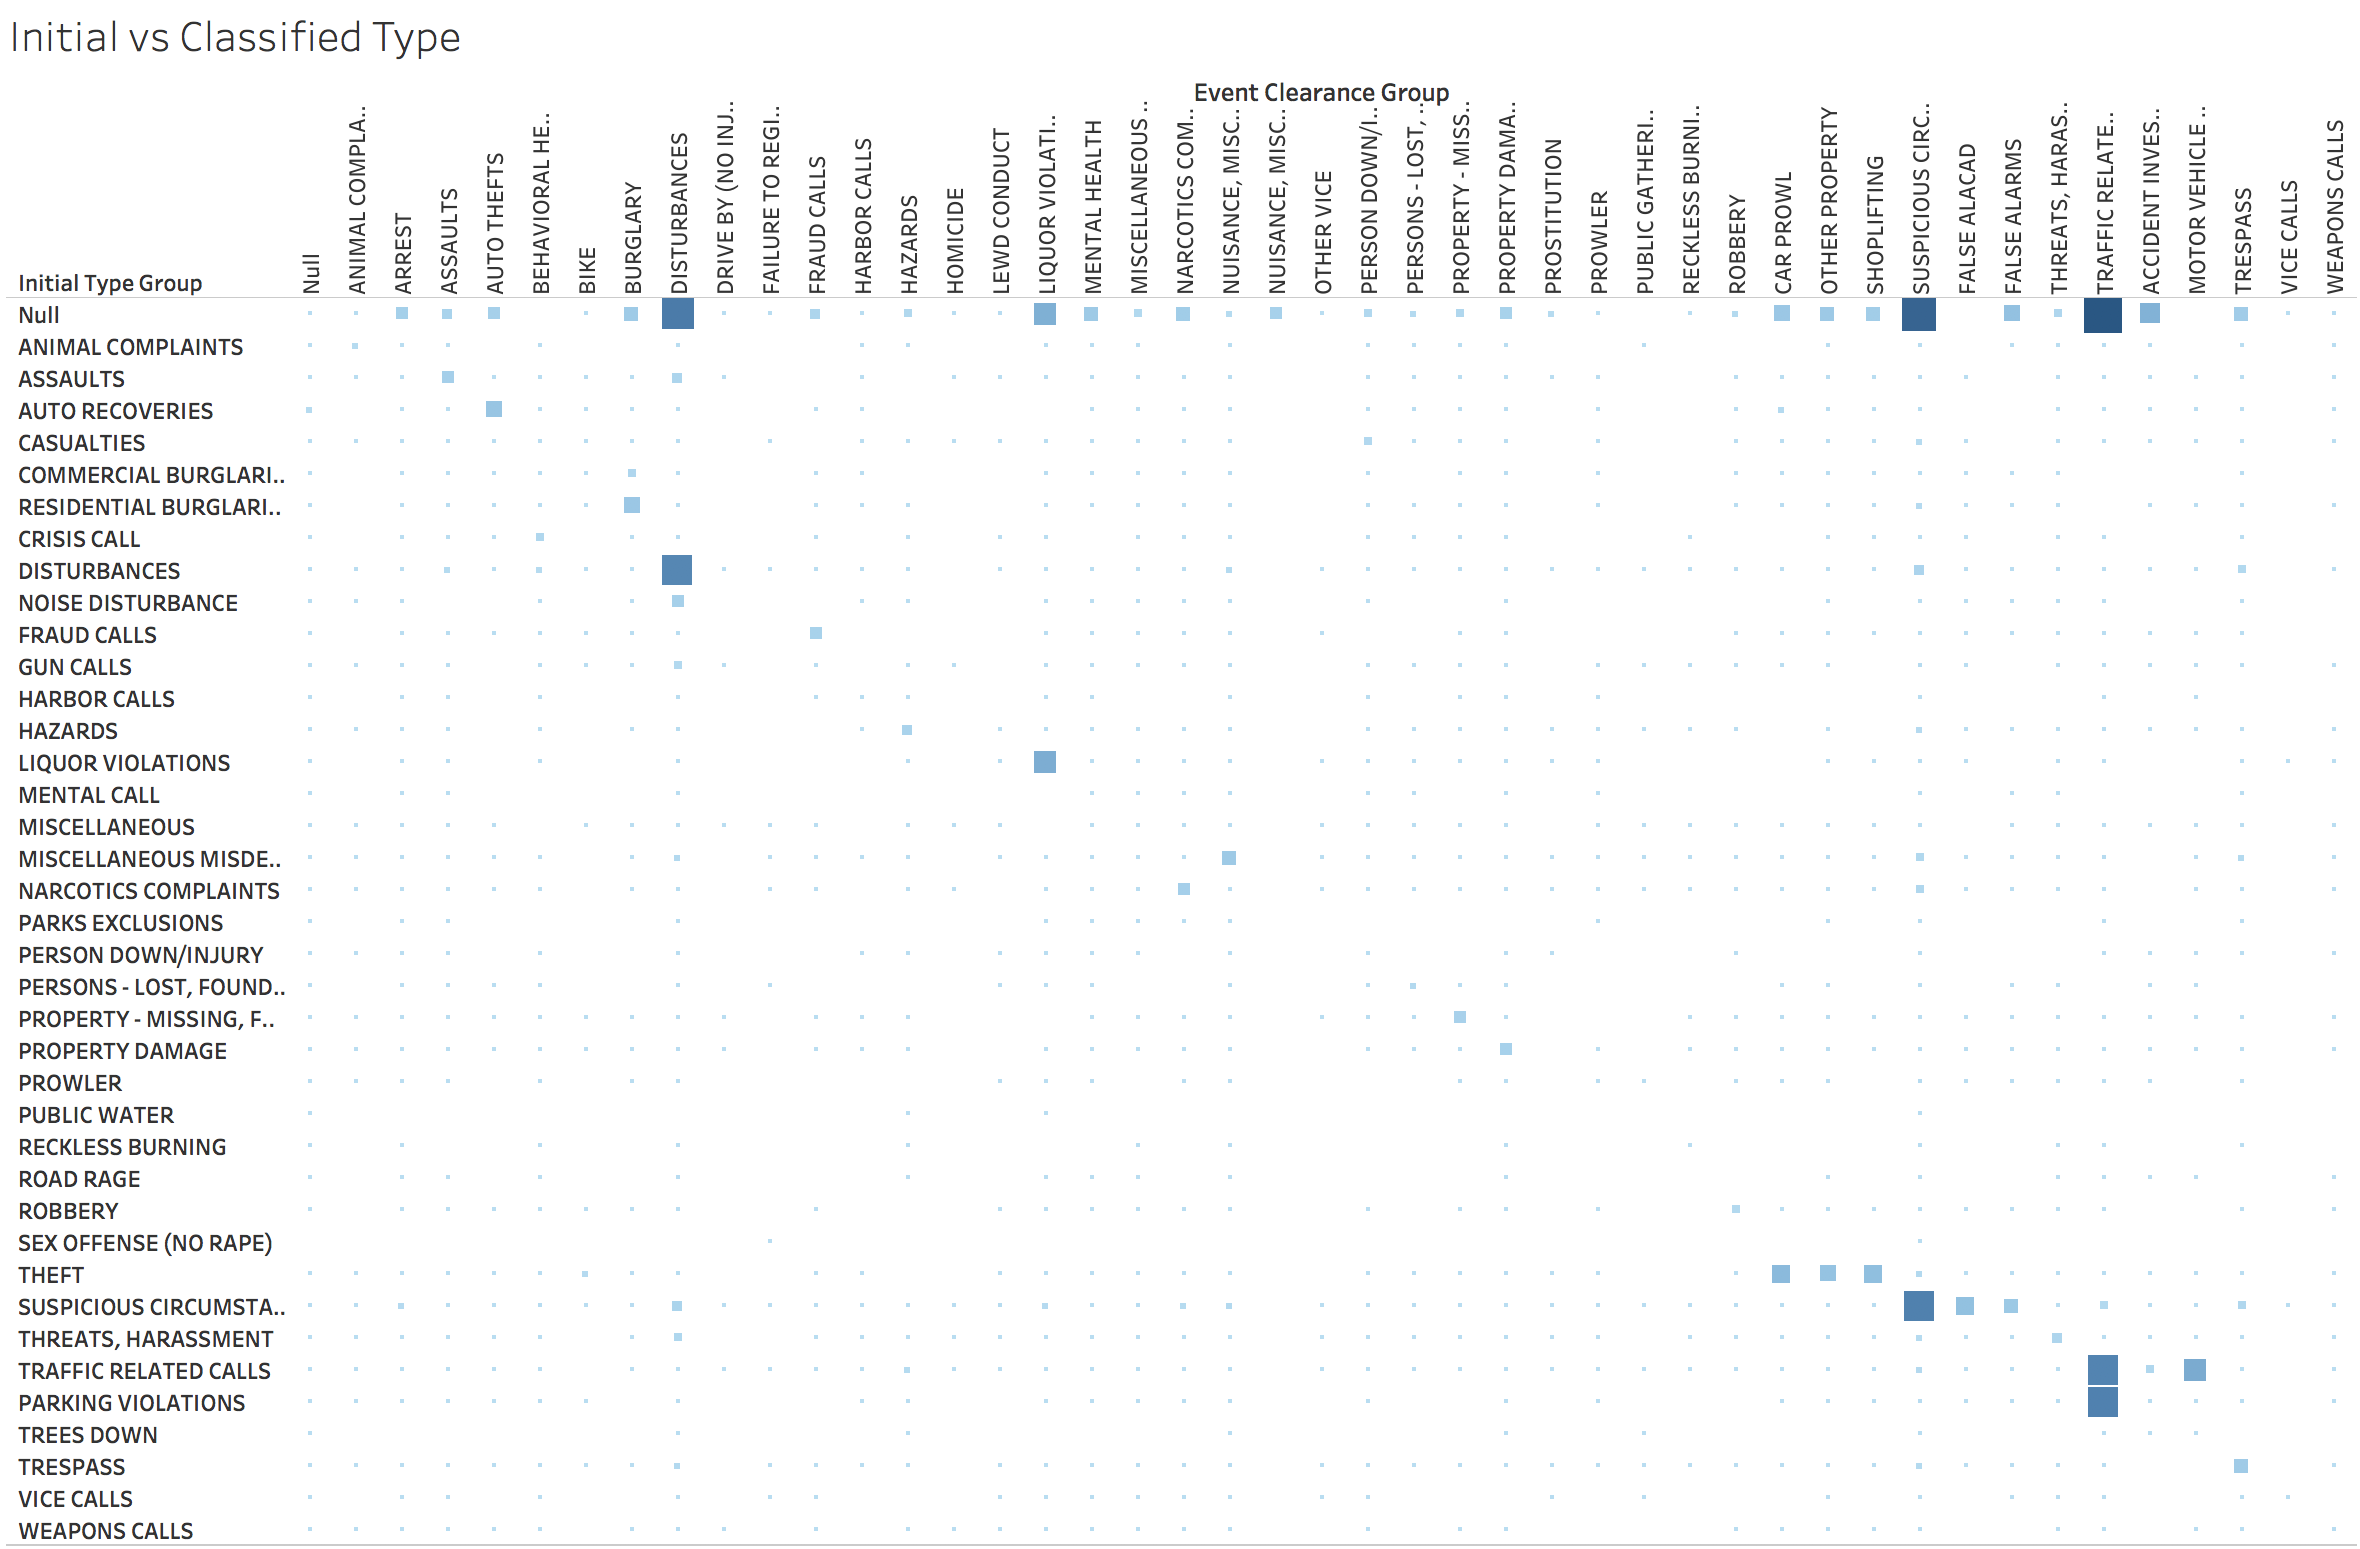
\includegraphics[width=\columnwidth]{figures/4_1_initial_vs_final_group_heatmap}
	\caption{Correlation between the initial and final incident type. The sheet is called ``Initial vs Final Type'' in Tableau.}
	\label{fig:4_1_initial_vs_final_group_heatmap}
\end{figure}

The visualization answers the question, but requires some manual work to find the matching between initial and final types.
Moreover, since most initial types are highly correlated to only a few final ones, it wastes a lot of space.
This makes the square dedicated to interesting correlations very small and difficult to compare with the others.
The use of colors as an overloading helps with that, by does not really solve the problem. 

To better visualize the interesting correlations and remove the manual reordering step, we use a treemap.
We filter out values without an initial type since we have discussed this case previously.
We use the initial type for the first split for the treemap.
Each rectangle corresponds to a pair initial and final types.
Both color and the area of each rectangle encode the number of elements for the particular pair.
Tooltips allows the user to interactively get additional information for each rectangle, namely initial type, final type and number of matching incidents.

\begin{figure}[h]
	\centering
	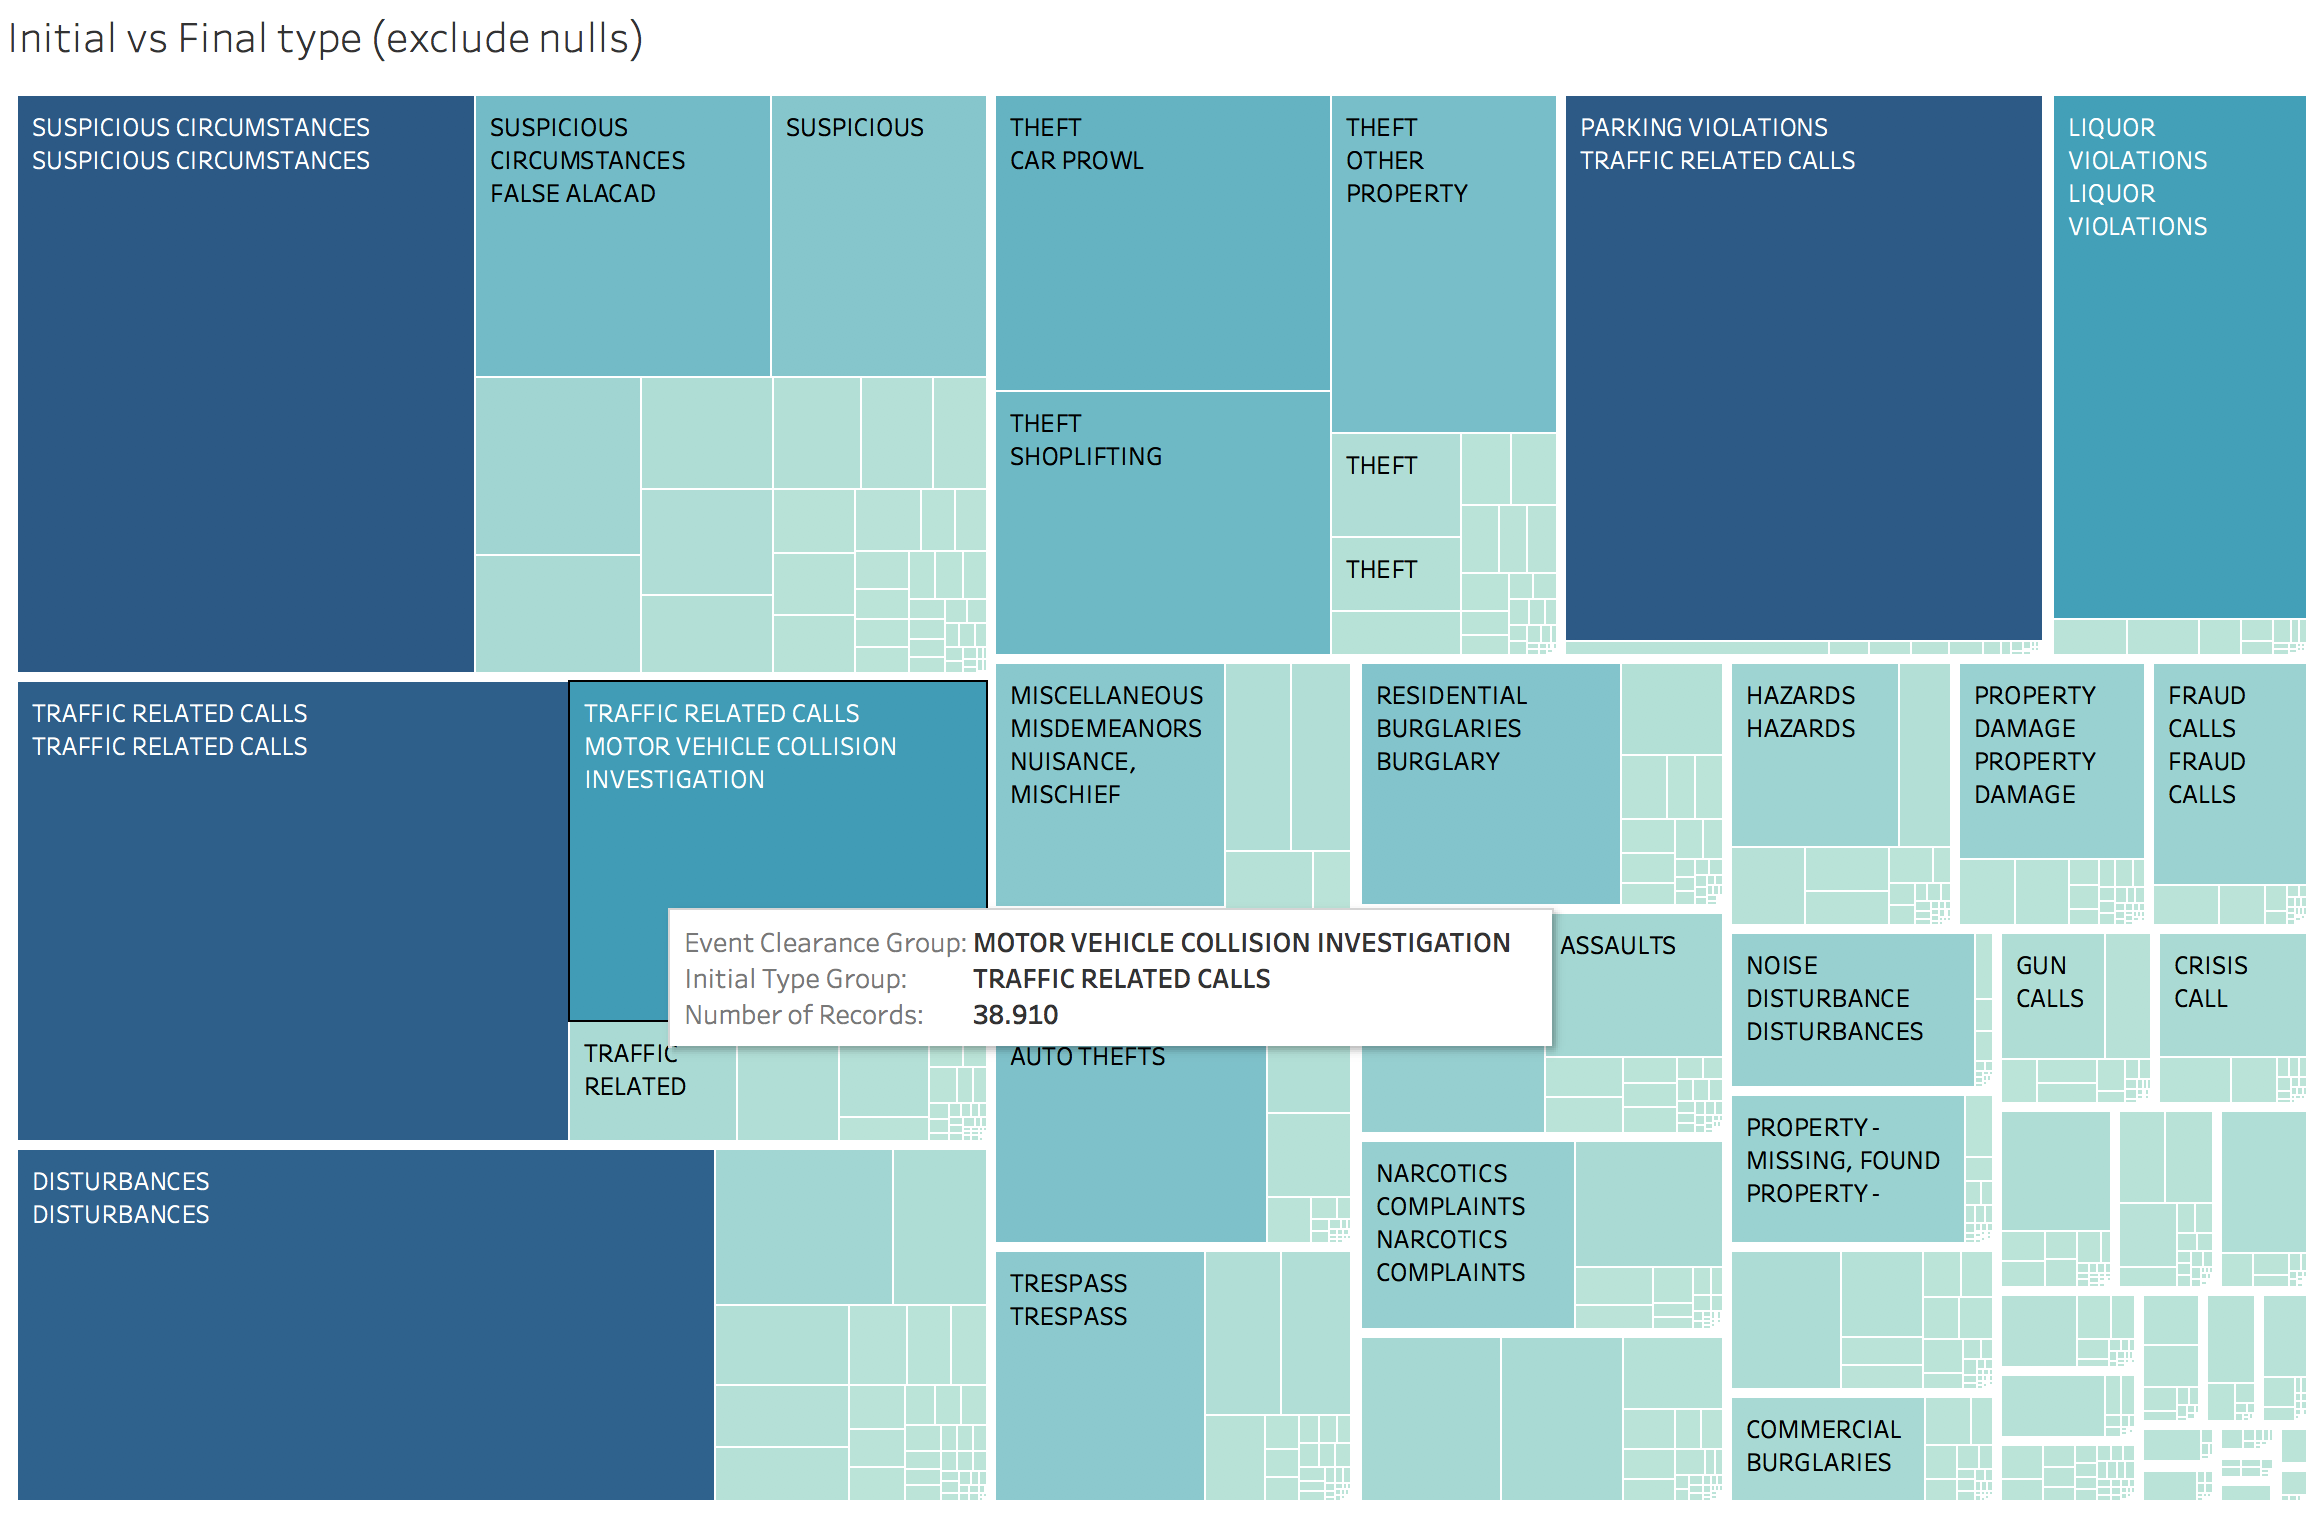
\includegraphics[width=\columnwidth]{figures/4_1_initial_vs_final_group_treemap}
	\caption{Correlation between the initial and final incident type (excluding incidents without an initial type). The sheet is called ``Initial vs Final Type (exclude nulls)'' in Tableau.}
	\label{fig:4_1_initial_vs_final_group_treemap}
\end{figure}

\cref{fig:4_1_initial_vs_final_group_treemap} shows the visualization:
\begin{itemize}
	\item There are some very big rectangles, which indicates a high correlation between the initial and final types.
	\item There are many small rectangles, which indicates a low correlation. For most types the area occupied from small rectangles is negligible, but for some other (e.g. \textit{Suspicious circumstances}) this area is quite relevant. This fact was very difficult to spot in the previous visualization.
	\item Mapping between the initial and final types do not need to be specified interactively by the user. This is the biggest improvement over the previous design.
\end{itemize}

To sum up, there is a quite strong correlation between initial and final types.
However, a lot of incidents with some particular initial cases are often classified in a different way afterwards (e.g. \textit{Suspicious circumstances}).

\subsection*{Question 4.2}
\textit{How do the total number of incidents break down per incident reported type (Initial Type Group) and incident resolution type (Event Clearance Group)?}

% To answer this question we can use the visualization build for the previous questions (see \cref{fig:4_1_initial_vs_final_group_treemap}):
% \begin{itemize}
% 	\item There are $5$ main types of 
% \end{itemize}

\subsection*{Question 4.3}
\textit{How do the total number of incidents break down per incident resolution type (Event Clearance Group) and incident resolution subtype (Event Clearance Subgroup)?}

Since groups and subgroups can be organized in a tree hierarchy, the visualization uses a treemap.
Each group is represented by a rectangle, which can be divided in sub-rectangles to represent the subgroups, if any.
Both color and size (area) encode the number of incidents with the given type / subtype.

\begin{figure}[h]
	\centering
	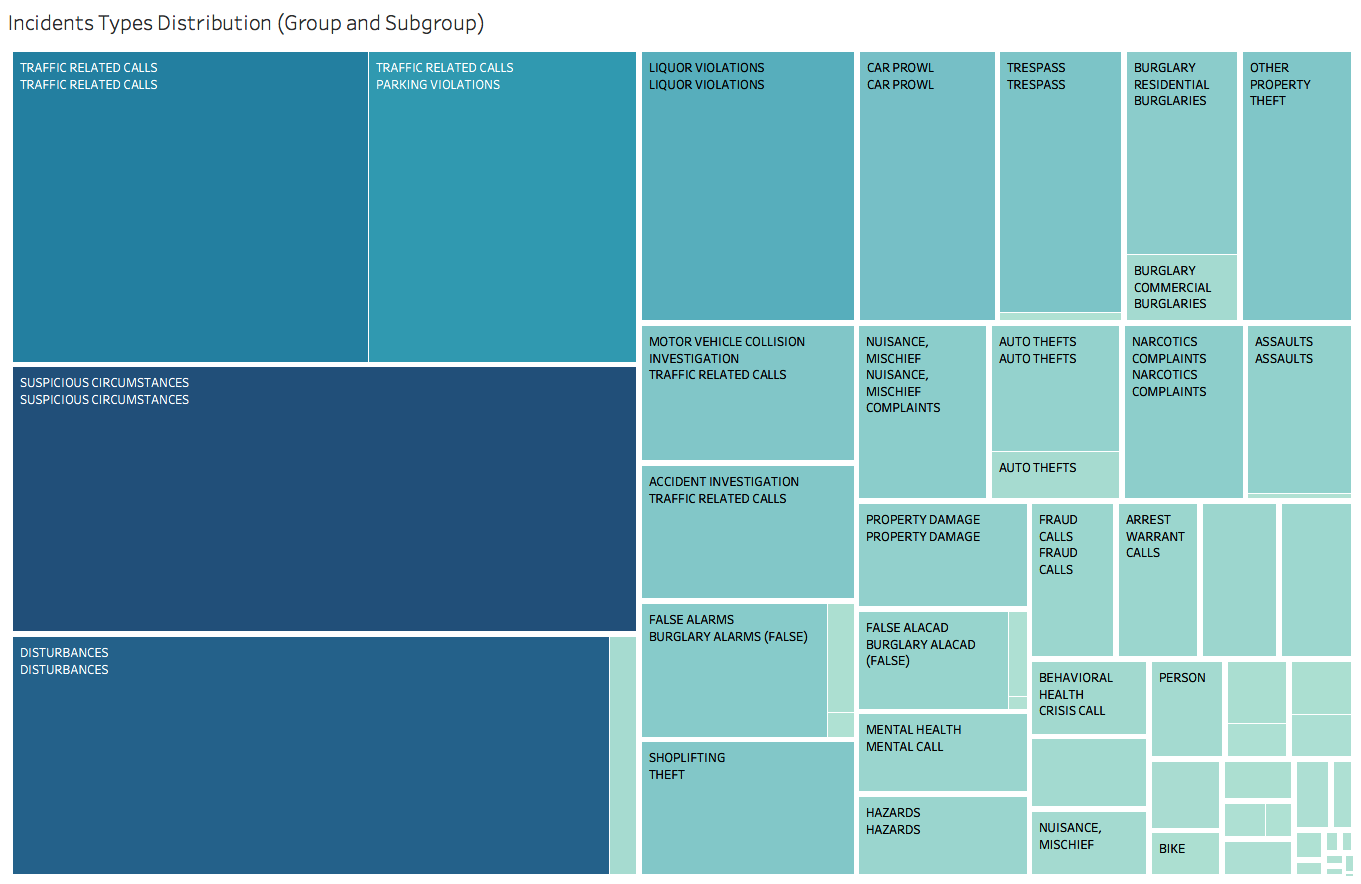
\includegraphics[width=\columnwidth]{figures/4_3_groups_subgroups}
	\caption{Incidents by Type and Subtype. The sheet is called ``Incidents Types Distribution (Group and Subgroup))'' in Tableau.}
	\label{fig:4_3_groups_subgroups}
\end{figure}

\cref{fig:4_3_groups_subgroups} shows the visualization.
We can see that:
\begin{itemize}
	\item There are $4$ types that include about $50\%$ of all of incidents, namely \textit{Traffic Related Calls}, \textit{Suspicious Circumstances}, \textit{Disturbances} and \textit{Liquor Violations}.
	\item Only $10$ out of $45$ type groups have subtypes.
	\item Groups that are divided in subgroups have only $2$ or $3$ of them.
	\item In most cases there is a dominant subgroups that includes most of the cases; the only exception is the group \textit{Traffic Related Calls}, where incidents are distributed almost equally in both subgroups \textit{Traffic Related Calls} and \textit{Parking Violations}.
\end{itemize}


\section{Exploring the incidents' temporal distribution}

\subsection*{Question 5.1}
\textit{How do the different types of incidents (as represented by Event Clearance Group) vary in number over the different years? Do you see different types of incidents having the same temporal variation pattern over the same year(s)?}

\begin{figure}[h]
	\centering
	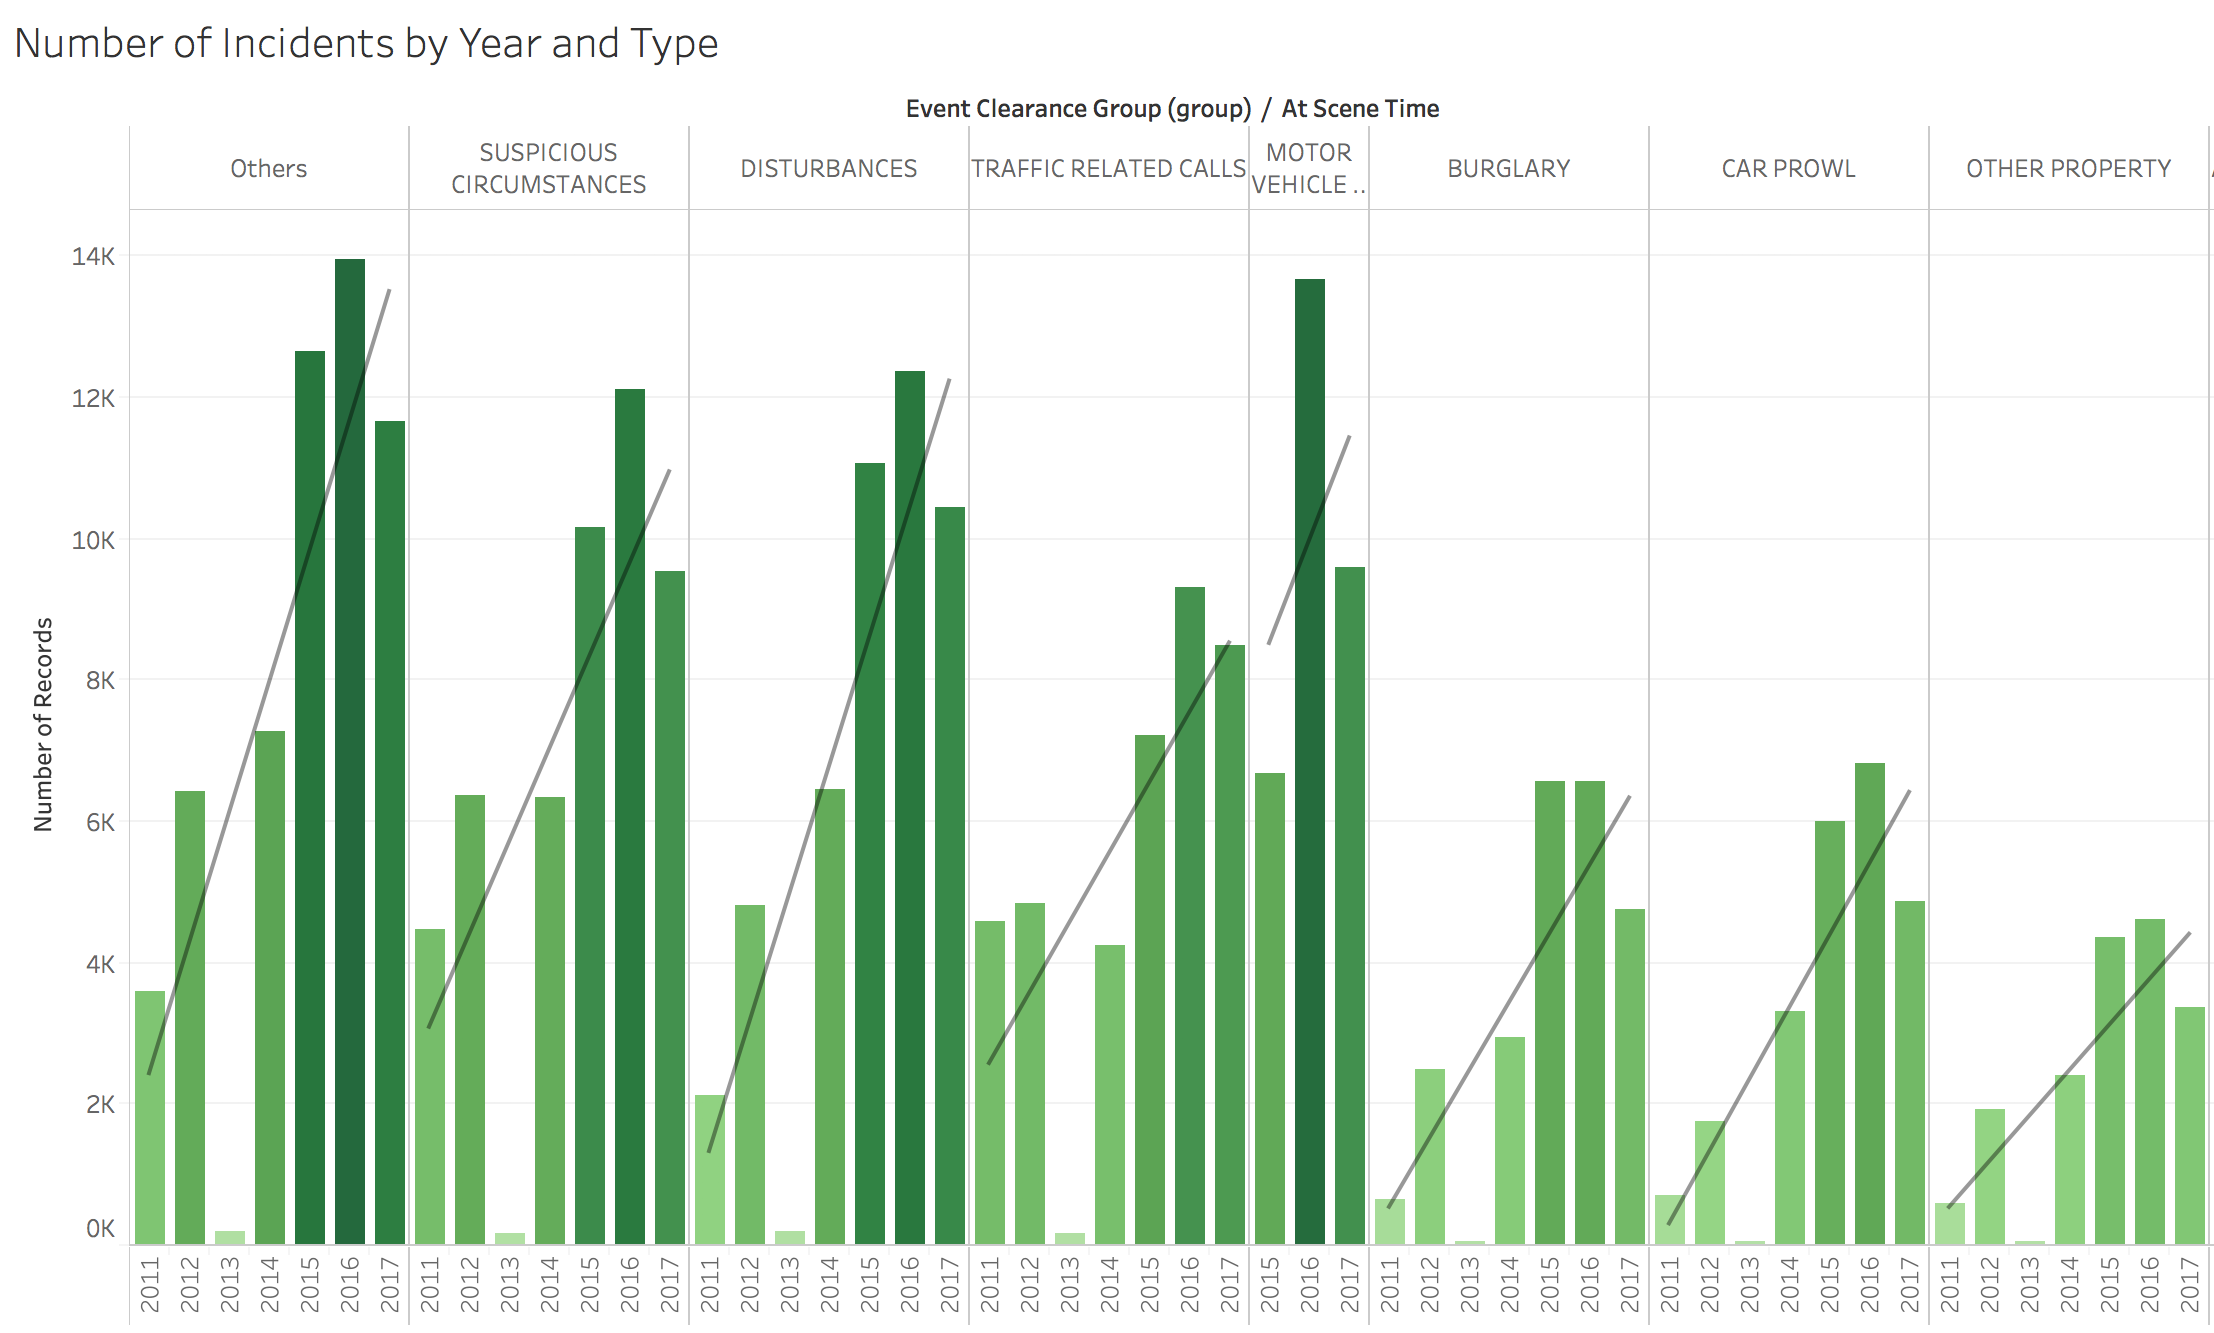
\includegraphics[width=0.9\columnwidth]{figures/5_1_incidents_by_type_and_year}
	\caption{Number of incidents by year and type. The sheet is called \textit{Number of Incidents by Year and Type} in Tableau.}
	\label{fig:5_1_incidents_by_type_and_year}
\end{figure}

The visualization uses bar charts and the small multiple design principle.
The x-axis represent the time (in years), while the y-axis encodes the number of incidents for the given year.
The bar chart is replicated for each incident type; bar charts for different types are organized in columns.
Color is used to overload the encoding of the number of incidents (showed by the y-axis).
Trend lines are drawn for each small bar chart to show the trend of the number of incidents over year for each different type.
The bar charts are ordered for the total number of incidents per type (decreasing).
The types with less incidents are aggregated together in the \textit{Others} group to spare space on the screen and thus better fit the visualization.
Since there are very few data for $2009$ and $2010$, those years are removed from the visualization.
We filter also null values for the date since we are interested in the trend of incidents over years.

\cref{fig:5_1_incidents_by_type_and_year} shows the visualization.
We can observe the following:
\begin{itemize}
    \item Only $2$ incidents' types decreased over time, namely \textit{Accident Investigation} and \textit{Mental Health}. For both types there is no single incident reported in years $2016$ and $2017$. We believe that this might be due to a change in the classification of incidents in types between $2015$ and $2016$.
    \item All other types of incidents showed an increase over time.
    \item Most incidents show a common pattern: there is an increase from $2011$ to $2012$ and a clear drop in $2013$; $2014$ has a about the same number of incidents as $2014$; years $2015$ and $2016$ have a fast increase, with the peak in $2016$; $2017$ has slightly less incidents than $2016$ (this is probably due to the missing data for the last $3$ months of 2017).
\end{itemize}

The visualization allows to answer the question.
However, it does not show the general trend of the incidents number over years.
To solve this problem, we created a second visualization using another bar chart.
The y-axis represents the incidents' types, the x-axis and color encode the number of incidents for the given year.
We use a continuous heatmap for the color, but a different color for the maximum value in comparison with the visualization in \cref{fig:5_1_incidents_by_type_and_year}.

\begin{figure}[h]
	\centering
	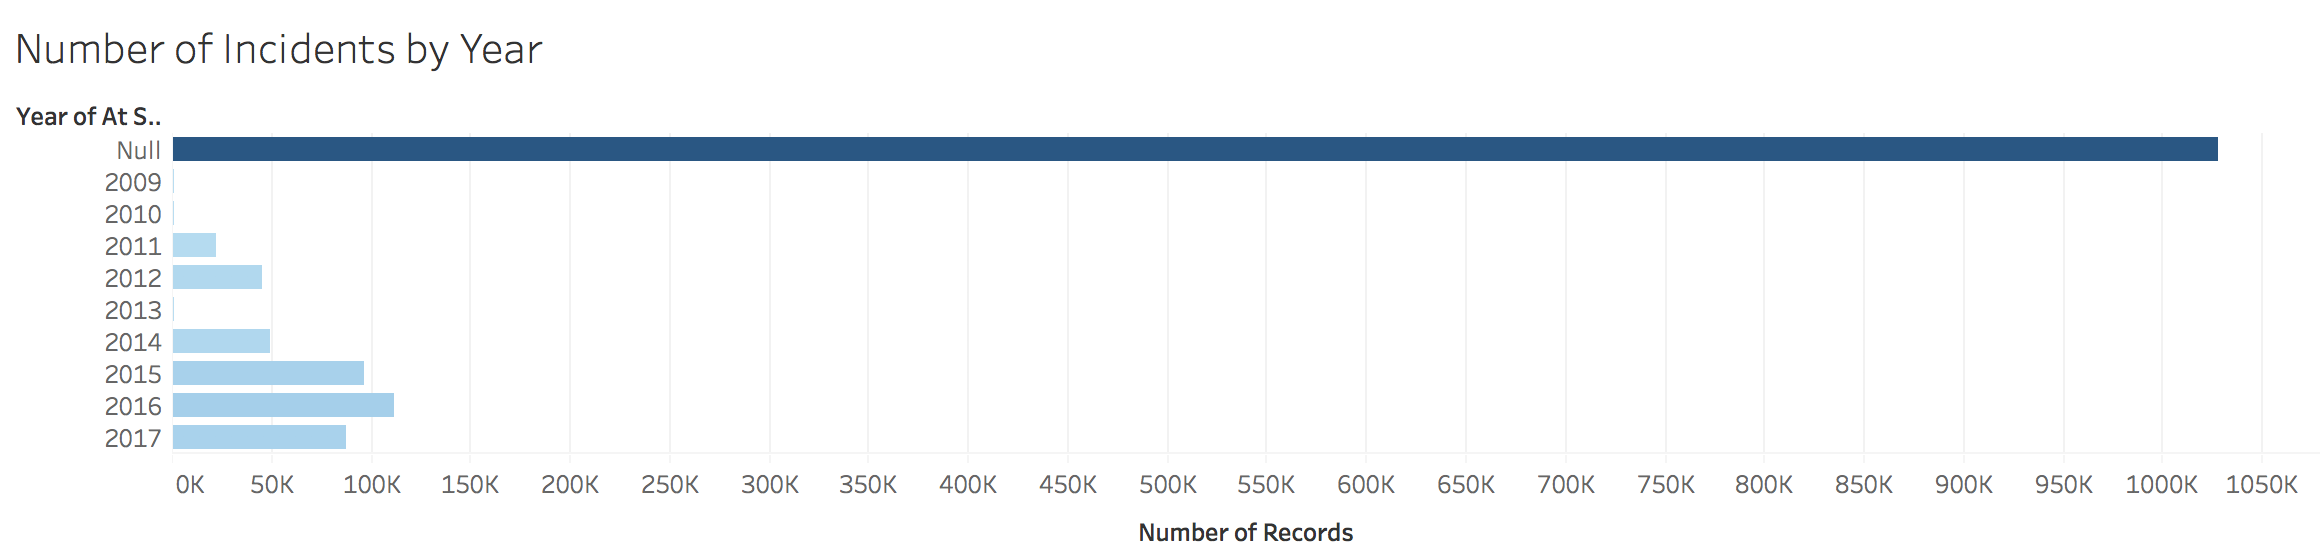
\includegraphics[width=0.9\columnwidth]{figures/5_1_incidents_by_year}
	\caption{Number of incidents by year. The sheet is called \textit{Number of Incidents by Year} in Tableau.}
	\label{fig:5_1_incidents_by_year}
\end{figure}

The visualization is showed in \cref{fig:5_1_incidents_by_year}.
We can notice that:
\begin{itemize}
    \item The majority of incidents in the dataset do not have the date information. The confident of the answer to the question is thus low.
    \item The general temporal distribution of incidents has the same trend of most incidents' types.
\end{itemize} 

The visualizations are grouped together in the \textit{Incidents Temporal Distribution by Type and Year} dashboard.


\subsection*{Question 5.2}
\textit{How do the different types of reported incidents (as represented by Initial Type Group) vary over the 24 hours of a day, for the entire data collection? Are there certain hours having a higher rate of reported incidents?}

The visualization uses bar charts and the small multiple design principle.
For each chart, the y-axis represent the hour of the day, while the x-axis and the color encode the number of incidents for the given hour.
The chart is replicated for each incident type, organized in columns.
The bar charts are ordered for the total number of incidents per type (decreasing, from left to right).
The types with less incidents are aggregated together in the \textit{Others} group to spare space on the screen thus better and fit the visualization and null values are filtered out.
We add the average line for each type in order to easier spot hours with more or less incidents than the average.

\begin{figure}[h]
	\centering
	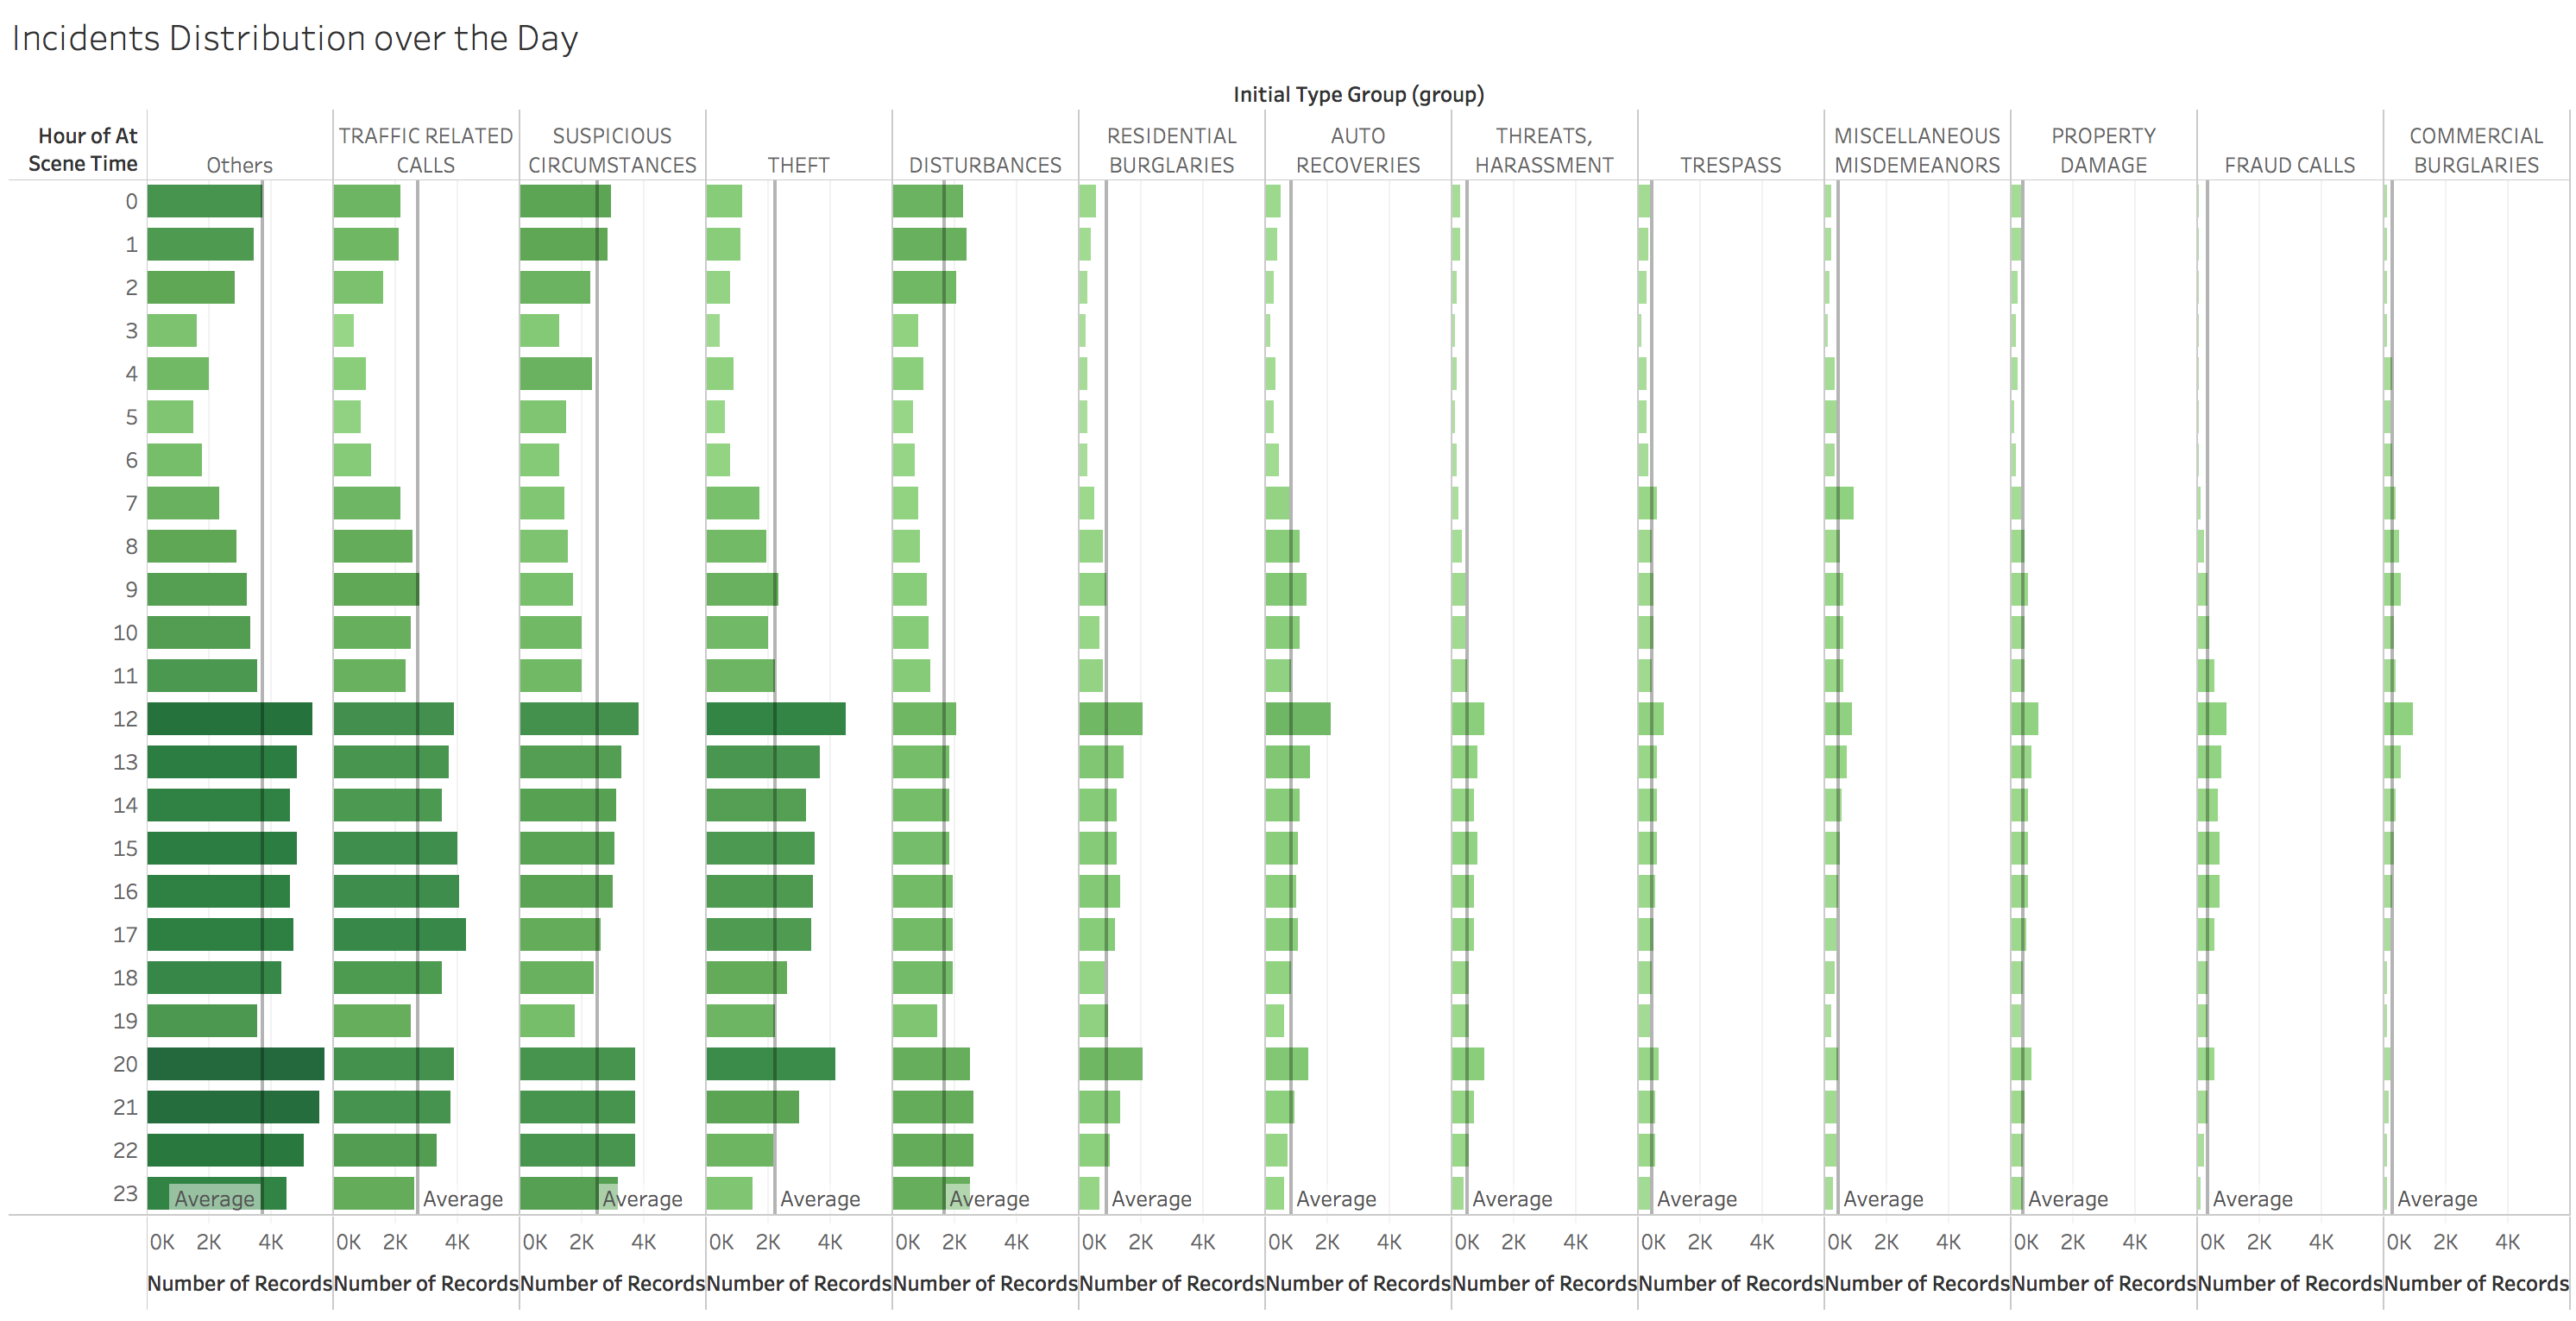
\includegraphics[width=\columnwidth]{figures/5_2_incidents_by_type_and_hour}
	\caption{Number of incidents by type over the different hours of the day. The sheet is called \textit{Incidents Distribution over the Day} in Tableau.}
	\label{fig:5_2_incidents_by_type_and_hour}
\end{figure}

From \cref{fig:5_2_incidents_by_type_and_hour} we can notice a common pattern among different types:
\begin{itemize}
	\item The number of incidents is generally smaller in the night / morning (23 - 11) and higher in the other hours.
	\item There are $2$ peaks, namely at $12$ and $20$: after these hours, incidents are still higher than the average but tend to gradually reduce in number.
	\item For most incidents the peaks have a similar number of incidents; there are a couple of exceptions, namely \textit{Fraud Calls} and \textit{Commercial Burglaries}, where the peak at $12$ is much higher than the one at $20$. 
\end{itemize}

\subsection*{Question 5.3}
\textit{How long does it take to clear incidents, as a function of the hour when they were reported? For example, do incidents reported at noon get cleared faster than incidents reported in the middle of the night?}

The visualization uses a bar chart.
The x-axis represents the hour of the day, while the y-axis shows the average resolution time for incidents reported in the given hour.
Color overloads the value showed in the y-axis.
The average line helps to compare particular time slots with the average behaviour.

Best practices for visualization suggests to use line charts instead of bar charts for continuous values like time.
In this case, however, we have discretized time into buckets of one hour and aggregated them together to compute the average.
In other words, we treat time as a discrete ordinal value.

\begin{figure}[h]
	\centering
	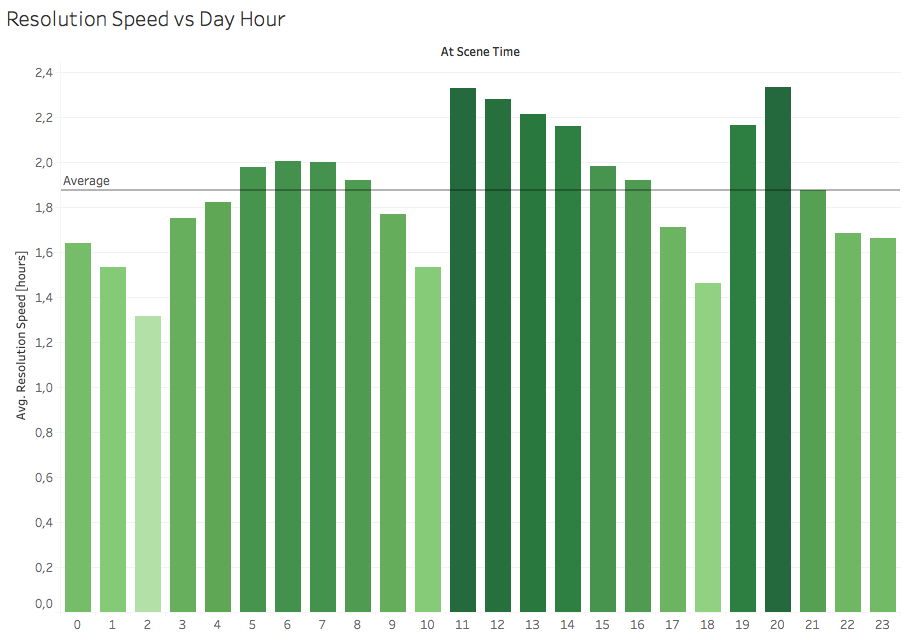
\includegraphics[width=0.9\columnwidth]{figures/5_3_resolution_speed_vs_hour}
	\caption{Resolution speed of incidents reported in different hour. The sheet is called \textit{Resolution Speed vs Day Hour} in Tableau.}
	\label{fig:5_3_resolution_speed_vs_hour}
\end{figure}

\cref{fig:5_3_resolution_speed_vs_hour} shows the visualization.
We can notice that:
\begin{itemize}
    \item The average time required to close incidents is not constant over the different hours of the day.
    \item Incidents that happens in the slots $11 - 14$ and $19 - 20$ take significant longer to be closed.
    \item Incidents that happens in the early morning ($5 - 7$) require on average more time than the incidents in the night and late morning ($9 - 10$).
    \item The time slots between $5 - 7$, $11 - 14$ and $19 - 20$ have a faster resolution speed.
\end{itemize}

To sum up, there is a correlation between the hour of the day and the time required to close incidents.
The visualization fully answers the question.

We have created a second visualization to check if this behaviour is common to all years.
The visualization uses again bar charts, one for each year.
The last column shows the average over all years as a reference for comparisons.
The axises are swapped in comparison to \cref{fig:5_3_resolution_speed_vs_hour} to better fit the screen.

\begin{figure}[h]
	\centering
	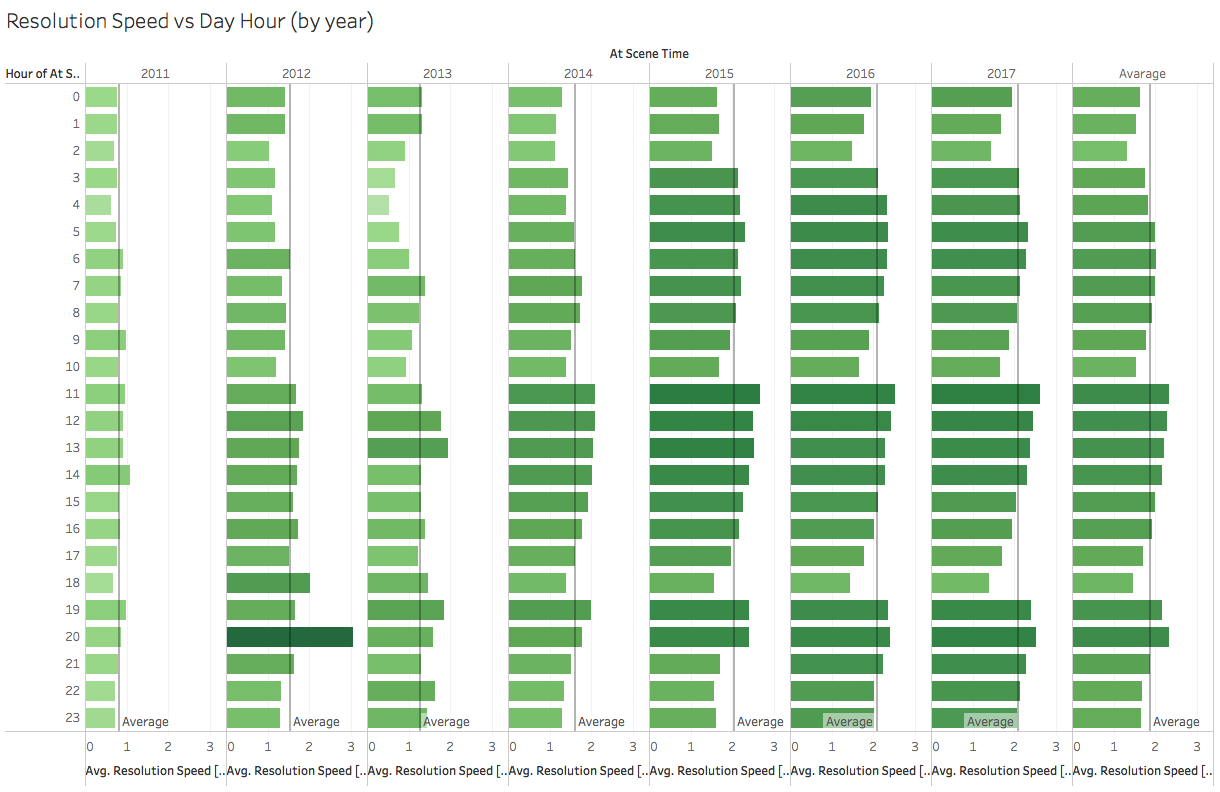
\includegraphics[width=0.9\columnwidth]{figures/5_3_resolution_speed_vs_hour_by_year}
	\caption{Resolution speed of incidents reported in different hour by year. The sheet is called \textit{Resolution Speed vs Day Hour (by year)} in Tableau.}
	\label{fig:5_3_resolution_speed_vs_hour_by_year}
\end{figure}

From \cref{fig:5_3_resolution_speed_vs_hour_by_year} we can notice that:
\begin{itemize}
    \item In $2011$ incidents are closed much faster than the average. There are some hours with a slightly higher resolution speed ($9$, $14$, $19$), but the difference with the rest of the day is small.
    \item Incidents that happens at $20$ in year $2012$ seems to take much longer to close than the average. This is probably due to the outliers discussed in \cref{sec:question3}, since both have very long resolution times and are in that slot of time.
    \item Years $2013$ have some picks in the slots $12 - 13$ and $18 - 20$. However, there are probably missing data for this year (see \cref{sec:question1}, so the confidence for this observation is low.
    \item Years $2014$, $2015$, $2016$ and $2017$ have a behaviour identical to the average over all years.    
\end{itemize}

To sum up, the resolution speed for the different hours of the day seems to be stable over years $2014$ to $2017$.
The previous years have slightly different behaviour, but still share some patterns.
Incidents that occurs in slots $5 - 7$, $11 - 14$ and $19 - 20$ take more time to be closed, while incidents between this slots are closed much faster.


% \bibliographystyle{IEEEtran}
% \bibliography{references}

\end{document}
